\documentclass{article}

\usepackage[utf8]{inputenc}
\usepackage[ngerman]{babel}
\usepackage[T1]{fontenc}

\usepackage{amsmath}
\usepackage{amssymb}
\usepackage{amsthm}
\usepackage{bbm}

\usepackage{geometry}
\geometry{a4paper,left=3cm,right=3cm,top=2.5cm,bottom=2.5cm}

\renewcommand{\baselinestretch}{1.45} 
\usepackage{setspace}

\usepackage{multicol}

\usepackage{graphicx} %use graph format
\usepackage{epstopdf}

%\usepackage{booktabs}

\title{Non-Paramatric Statistics Exercise 6}
\author{Osman Ceylan, Jiahui Wang, Zhuoyao Zeng}
\date{\today}

\begin{document}
\maketitle

\section*{Exercise 2.15} \vspace*{-1em}
Implement a kernel density estimator $D \mapsto h_{D,K,s}$, where $K$ may be the moving window, the triangular, the Epanechnikov, or the Gaussian kernel, and the used norm is either the Euclidean norm $||\cdot ||_2$ or the supremum norm $||\cdot ||_{\infty}$ on $\mathbb{R}^d$.\vspace*{1em} \\
\textit{Solution:} \\
Since there are no complexity requirement or other restrictions, we have  implemented the  $K$-mollification in a normal way and we don't think there is much to elaborate. \\
To visualize the implementation, we consider the distribution of the unit Euclidean ball in $\mathbb{R}^2$, because it is elementary and intuitive. The data set $D$ for generating $h_{K,D,s}$ has  10.000 points. For different kernel functions $K$, different norms $||\cdot ||$ and different $s$, we generate a set of equidistant grid points in the area $[-1.05 , 1.05]^2$, compute their respective values under $h_{K,D,s}$ and plot the result in squared scatters with the same scale of colour bars. \vspace*{1em}\\
Now we present some of our visualisation results. \\
Firstly, we demonstrate the results of Moving Window Kernel under different $s$ and different norms: \\
\hspace*{-1.5cm}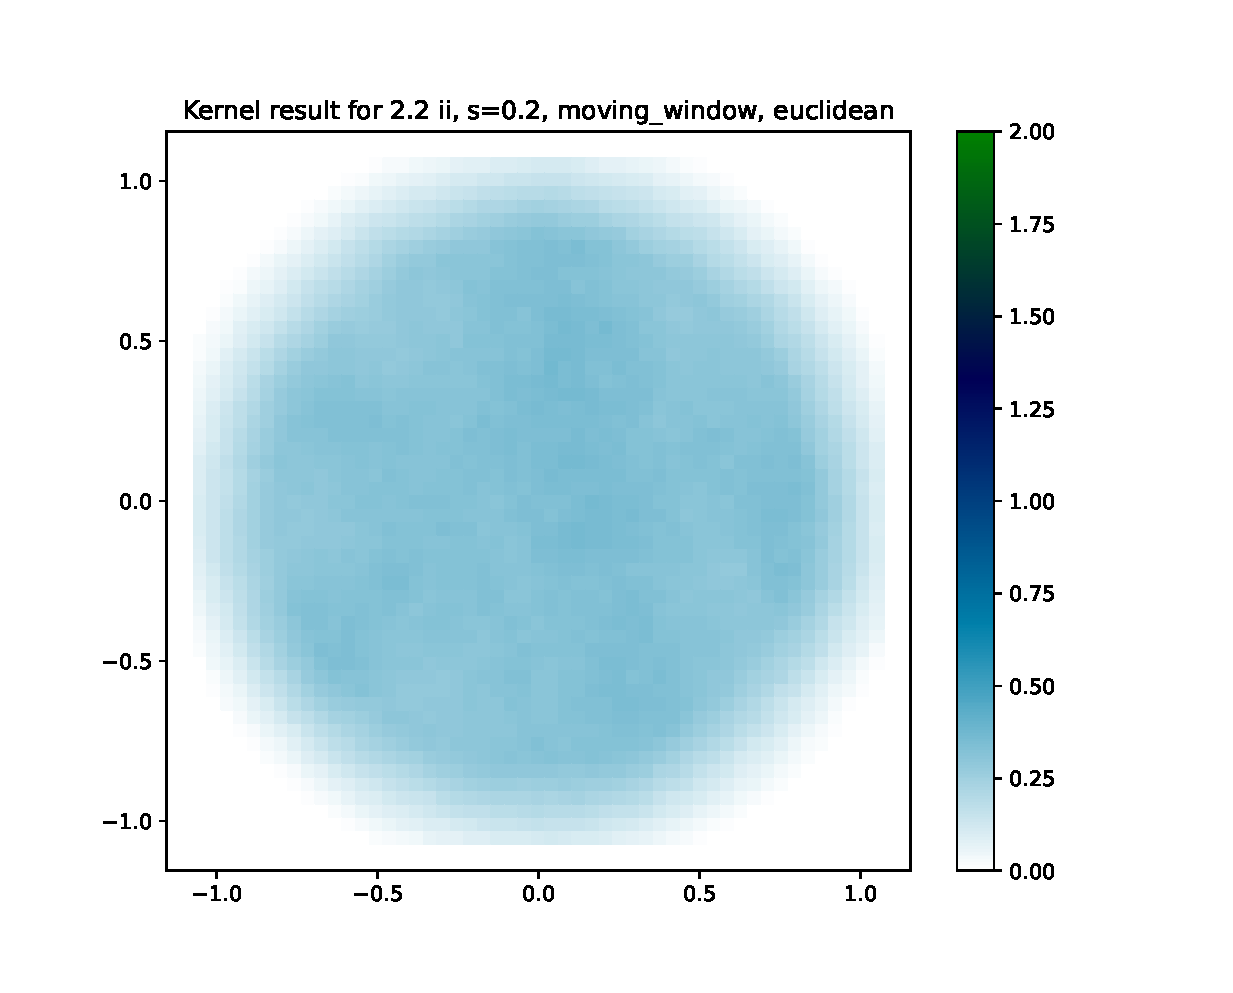
\includegraphics[height=8cm]{comparisons//Kernel_result_2-2ii_s_0-2_moving_window_euclidean.eps} \hspace*{-1.5cm}
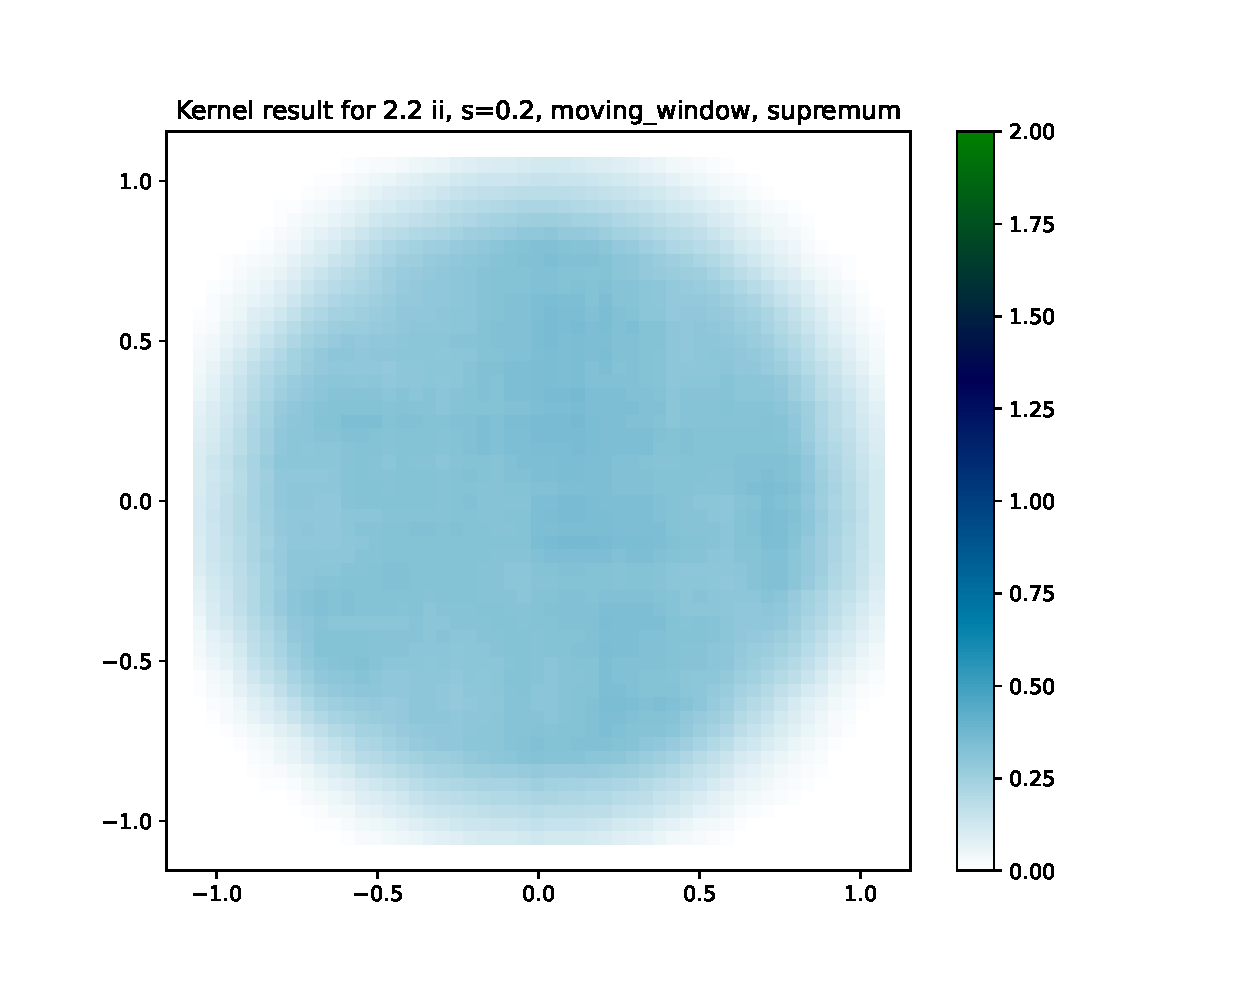
\includegraphics[height=8cm]{comparisons//Kernel_result_2-2ii_s_0-2_moving_window_supremum.eps} \\
\hspace*{-1.5cm}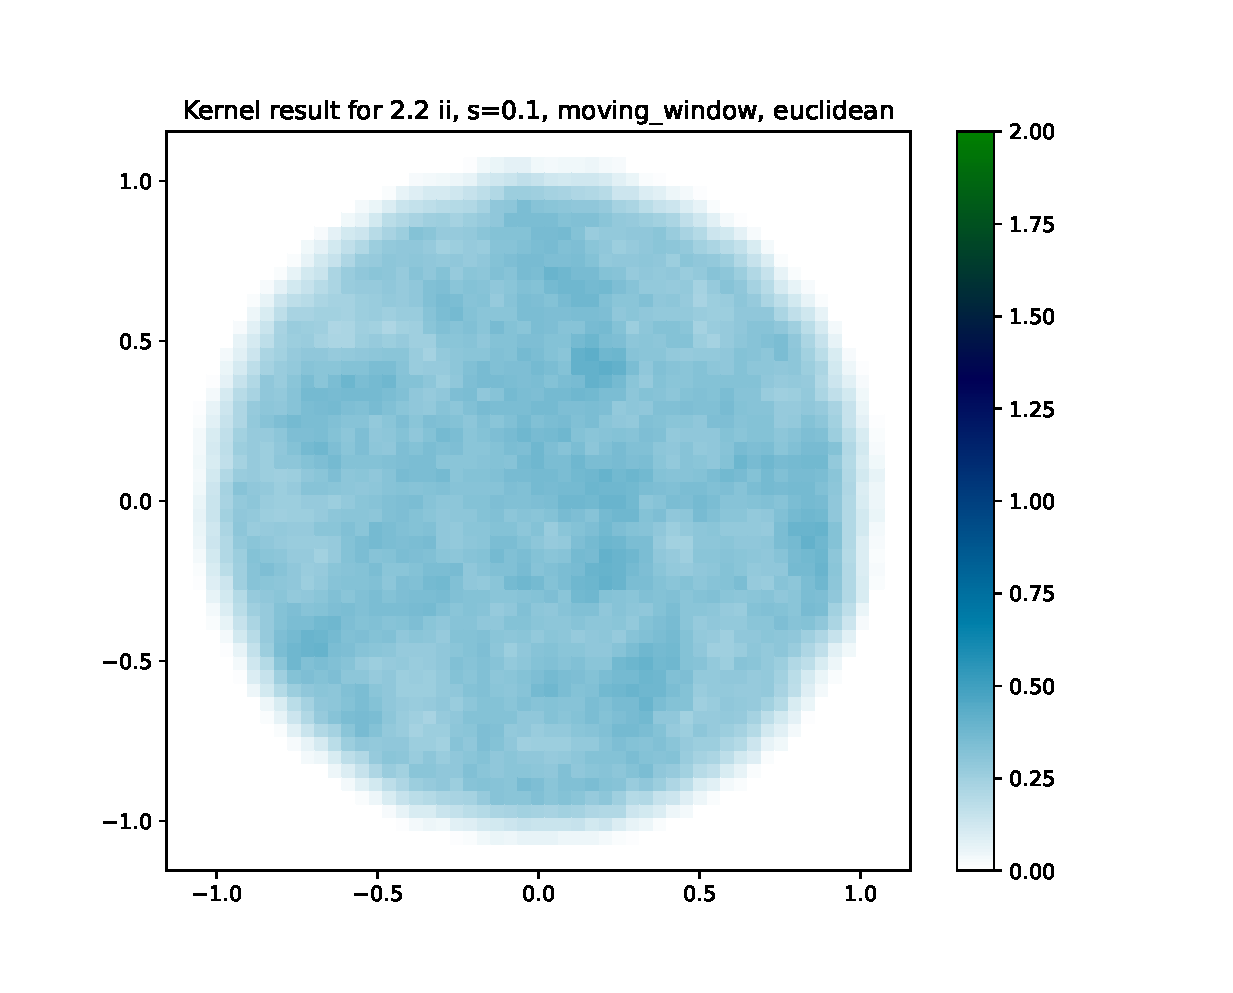
\includegraphics[height=8cm]{comparisons//Kernel_result_2-2ii_s_0-1_moving_window_euclidean.eps} \hspace*{-1.5cm}
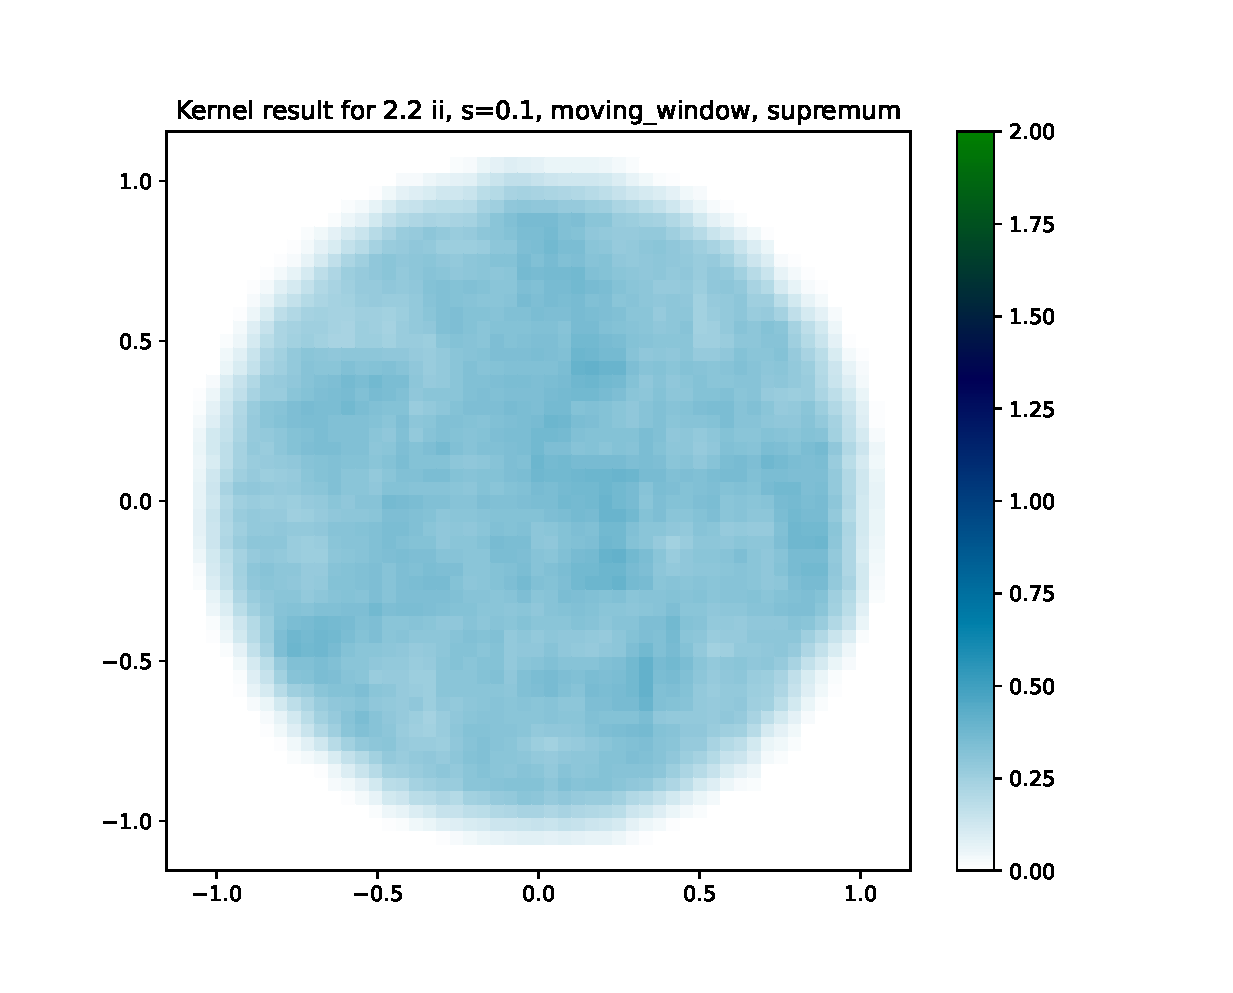
\includegraphics[height=8cm]{comparisons//Kernel_result_2-2ii_s_0-1_moving_window_supremum.eps}\\
\hspace*{-1.5cm}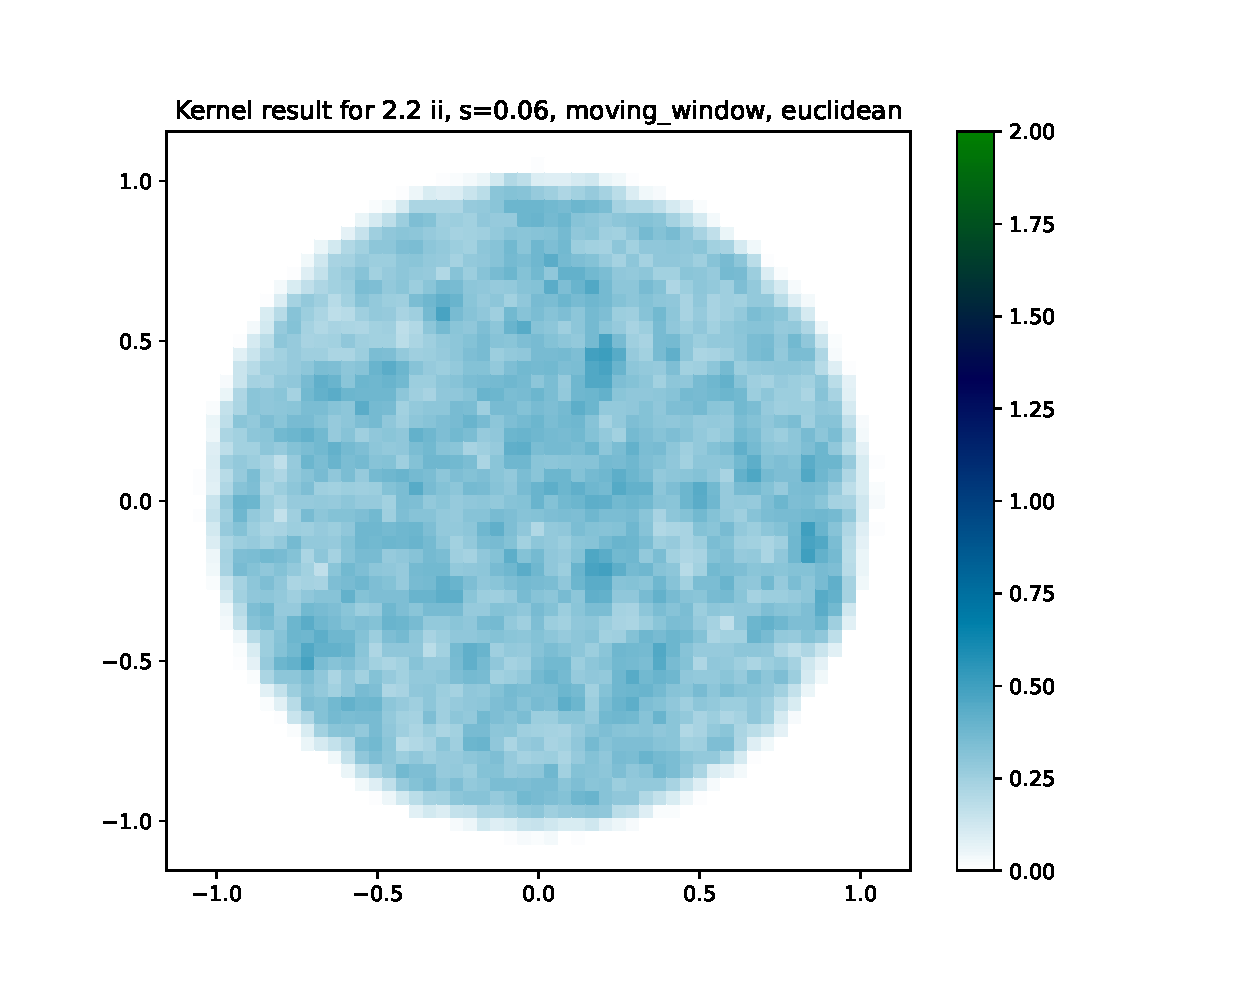
\includegraphics[height=8cm]{comparisons//Kernel_result_2-2ii_s_0-06_moving_window_euclidean.eps} \hspace*{-1.5cm}
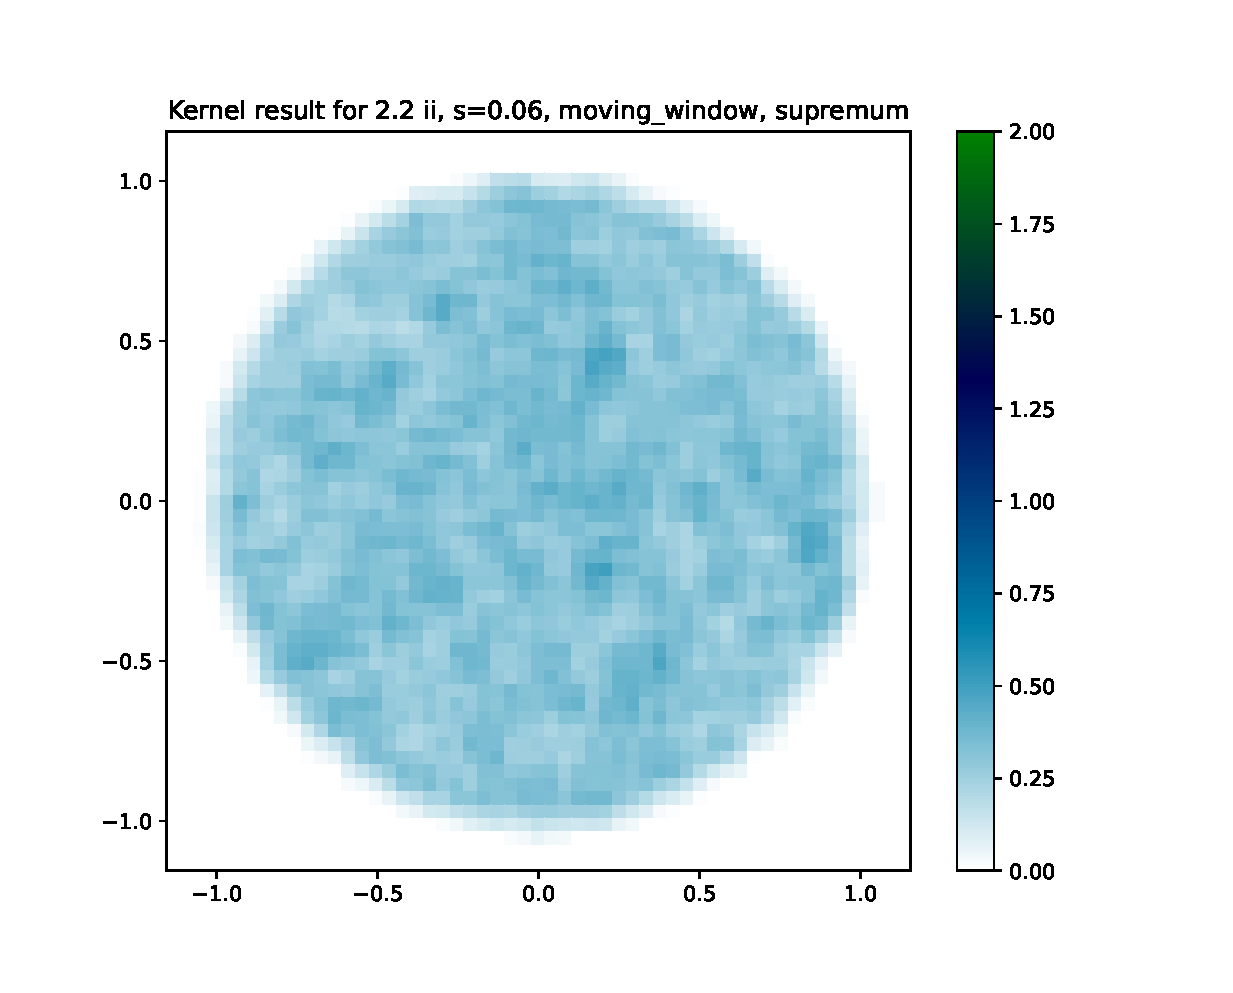
\includegraphics[height=8cm]{comparisons//Kernel_result_2-2ii_s_0-06_moving_window_supremum.eps}\\
\hspace*{-1.5cm}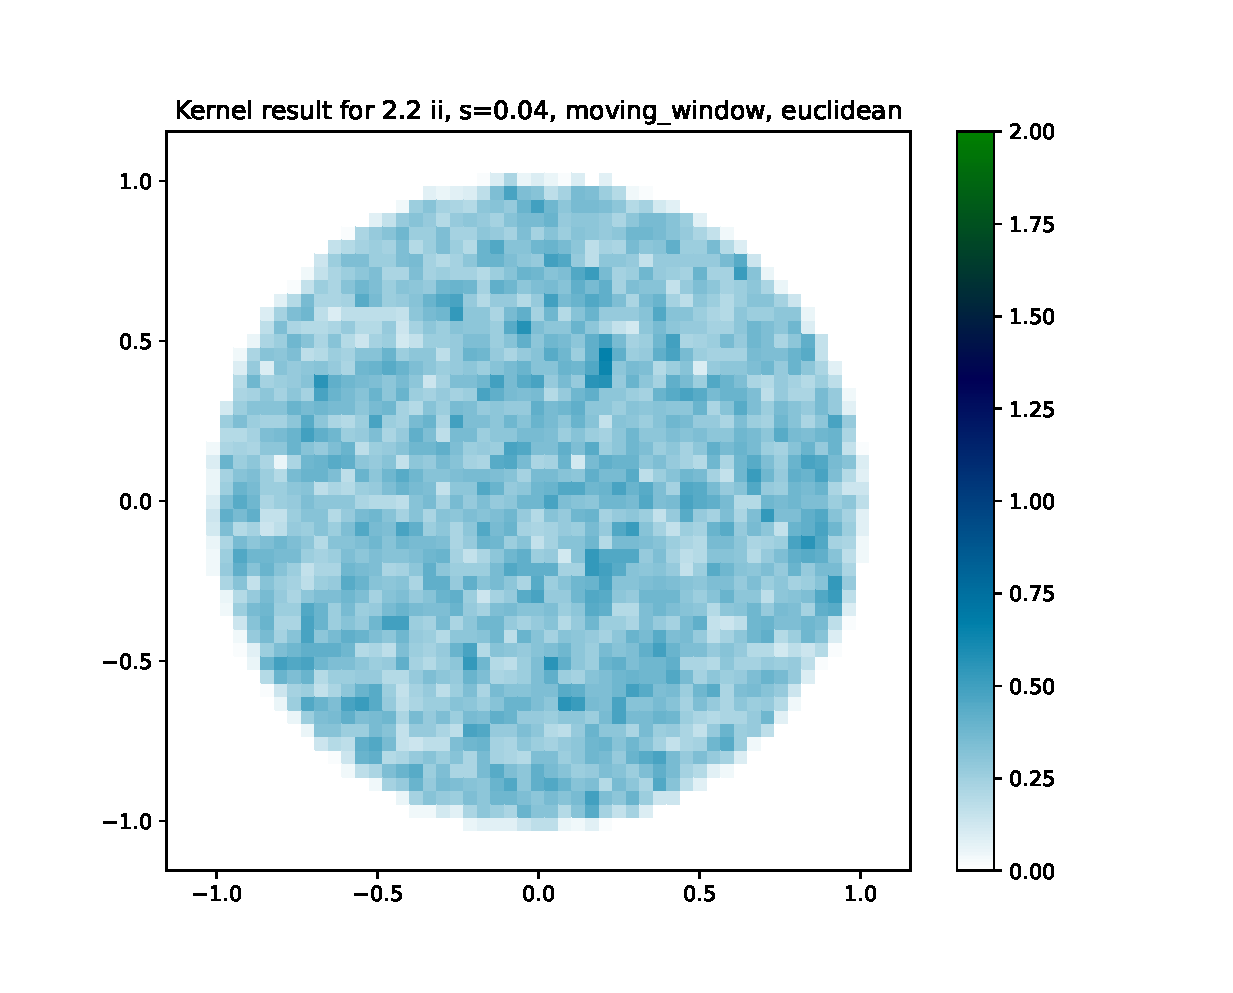
\includegraphics[height=8cm]{comparisons//Kernel_result_2-2ii_s_0-04_moving_window_euclidean.eps} \hspace*{-1.5cm}
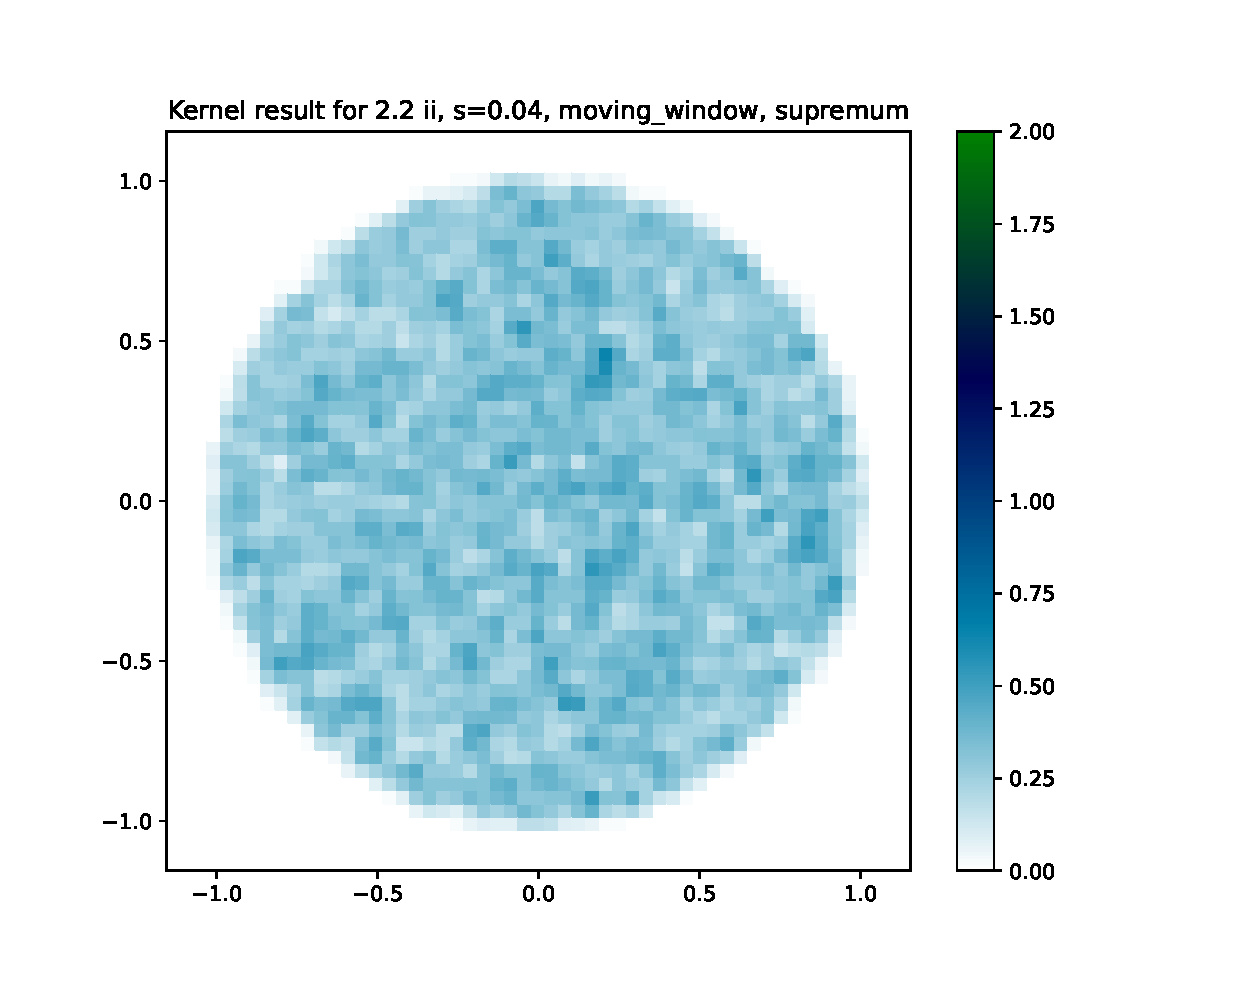
\includegraphics[height=8cm]{comparisons//Kernel_result_2-2ii_s_0-04_moving_window_supremum.eps}\\
\hspace*{-1.5cm}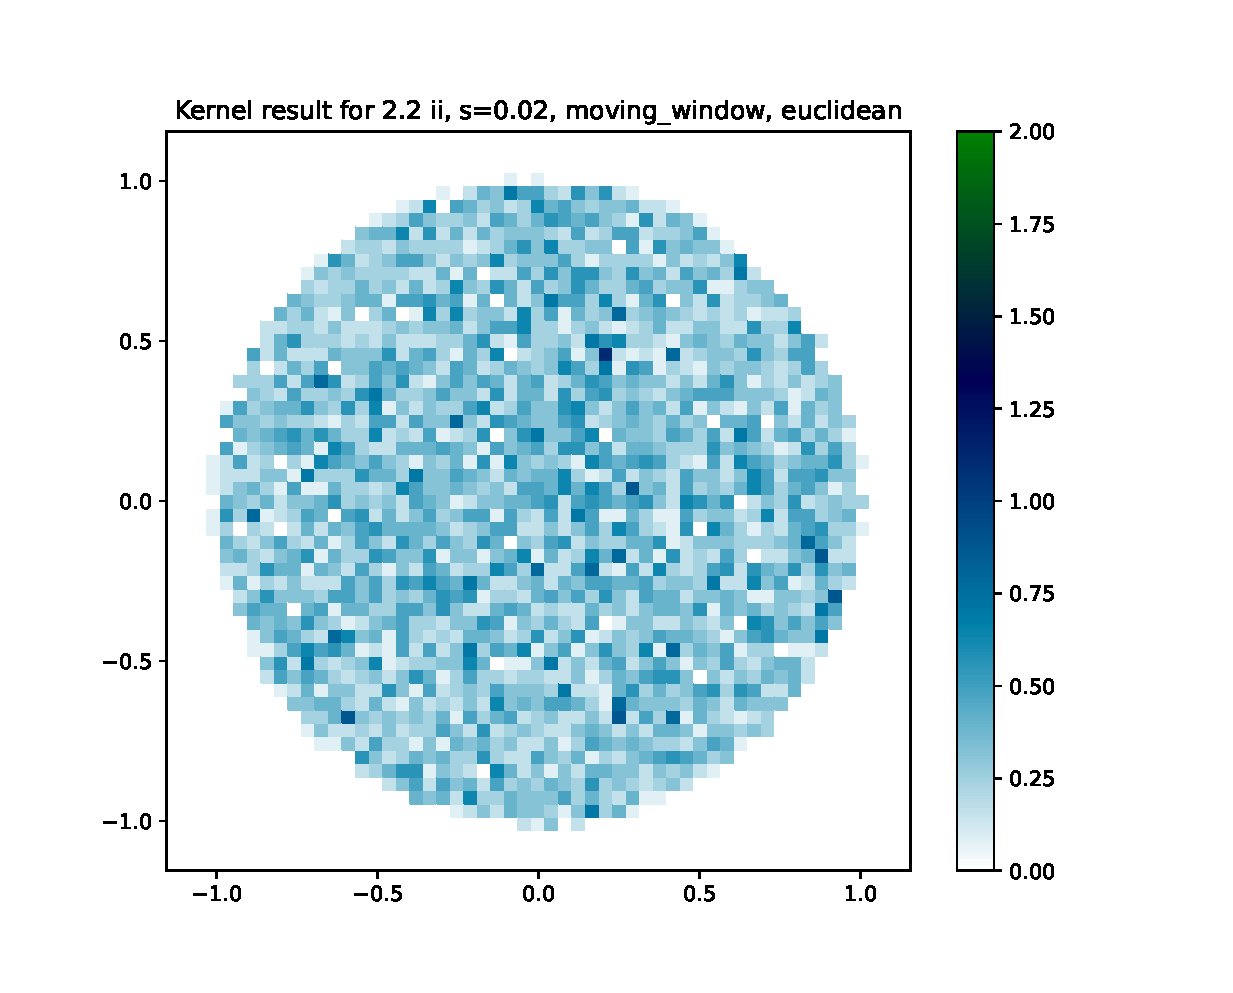
\includegraphics[height=8cm]{comparisons//Kernel_result_2-2ii_s_0-02_moving_window_euclidean.eps} \hspace*{-1.5cm}
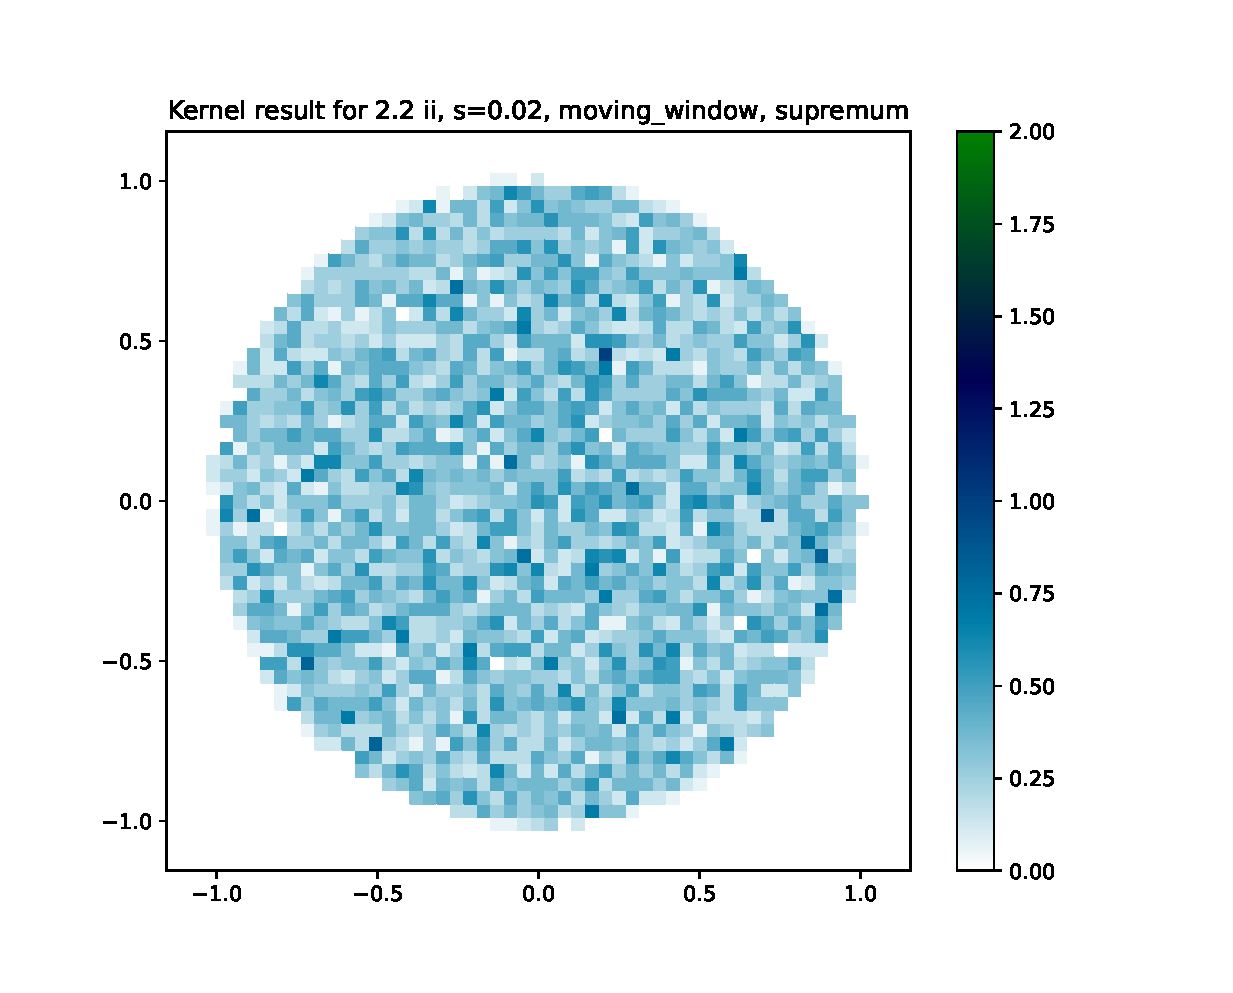
\includegraphics[height=8cm]{comparisons//Kernel_result_2-2ii_s_0-02_moving_window_supremum.eps}\vspace*{-1em} \\
\hspace*{-1.5cm}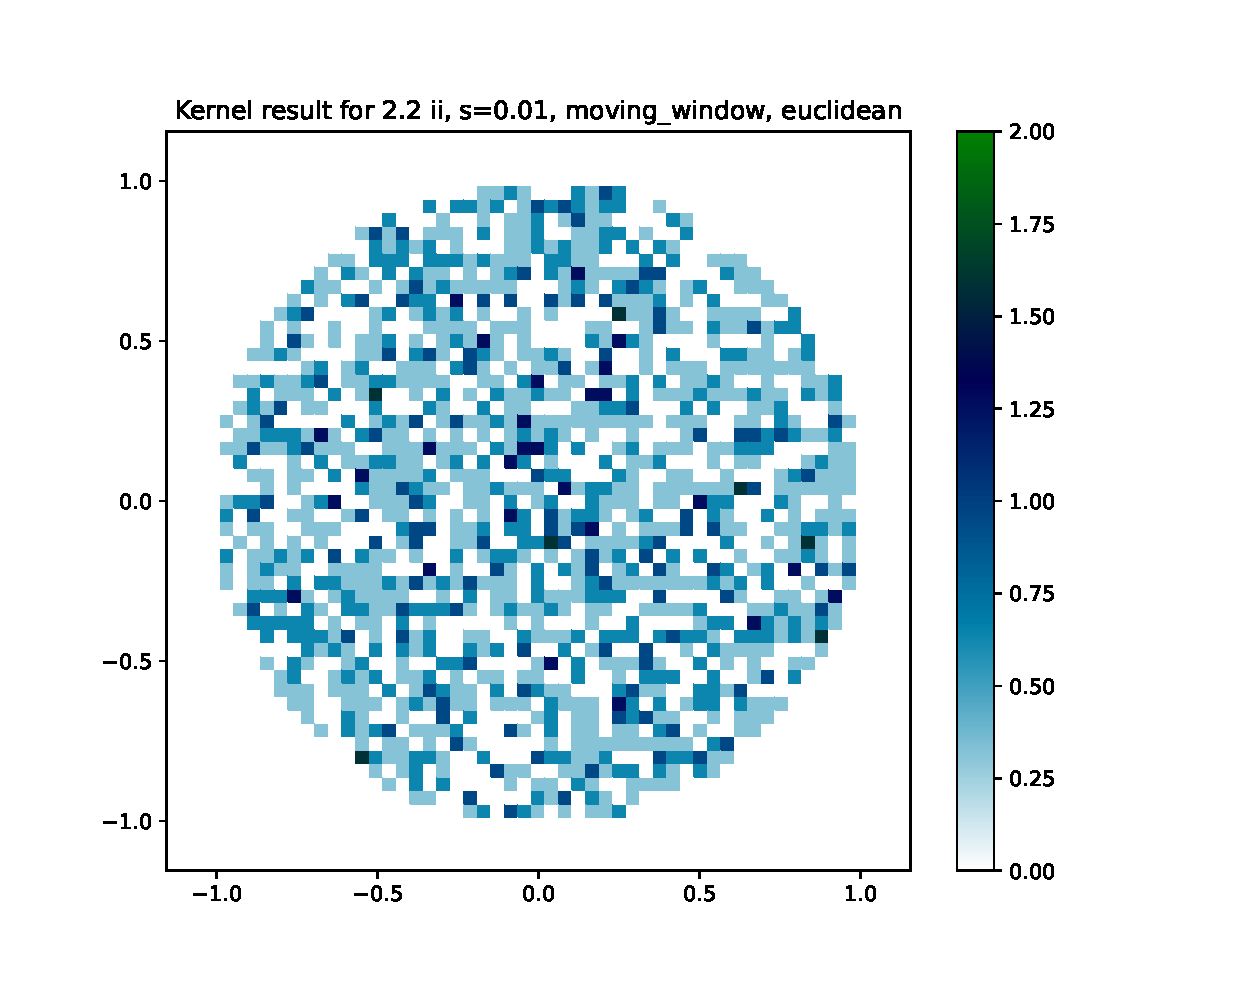
\includegraphics[height=8cm]{comparisons//Kernel_result_2-2ii_s_0-01_moving_window_euclidean.eps} \hspace*{-1.5cm}
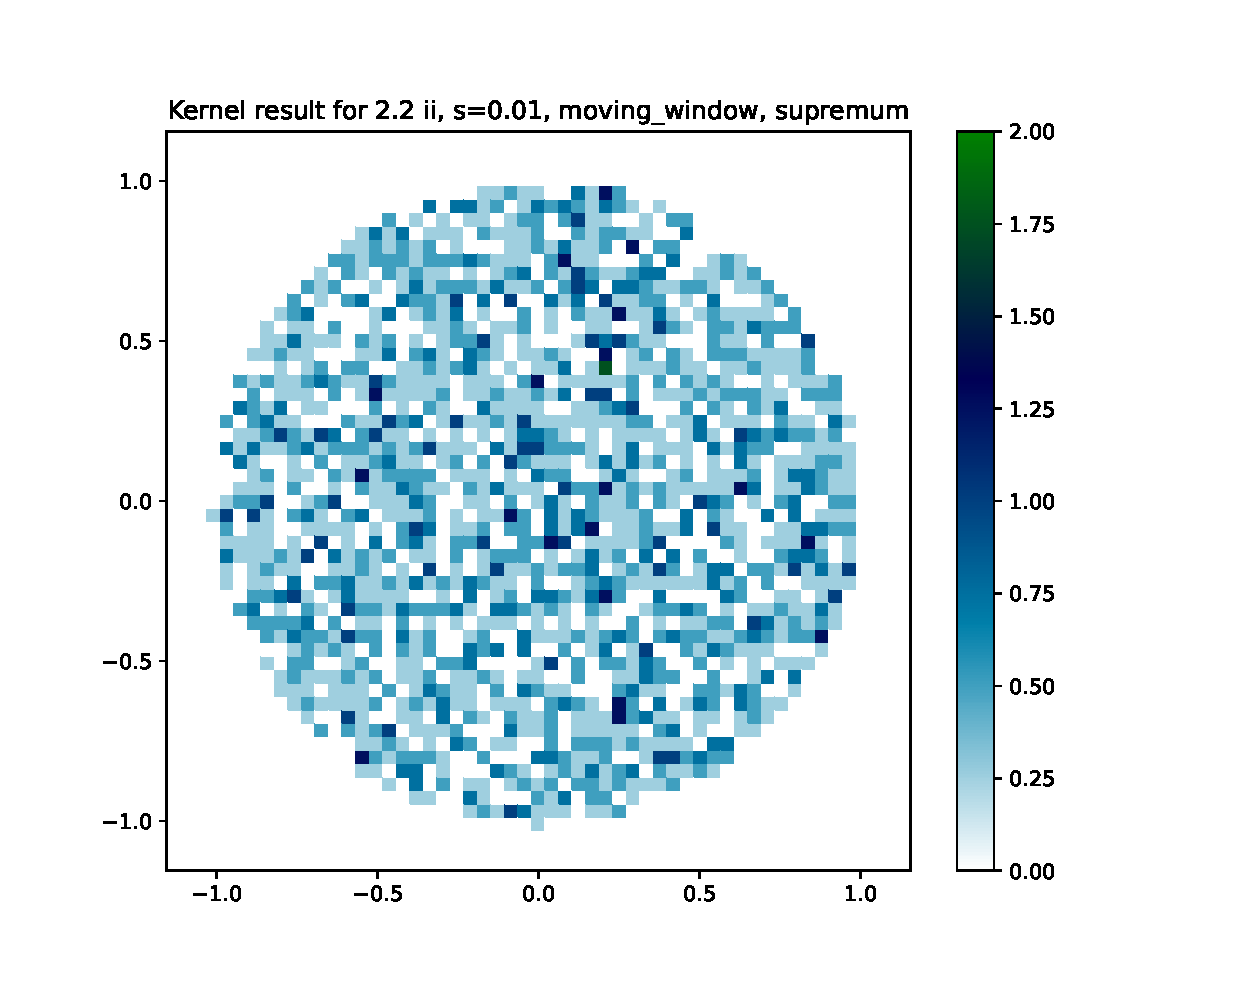
\includegraphics[height=8cm]{comparisons//Kernel_result_2-2ii_s_0-01_moving_window_supremum.eps} \vspace*{-2.5em} \\
\hspace*{-1.5cm}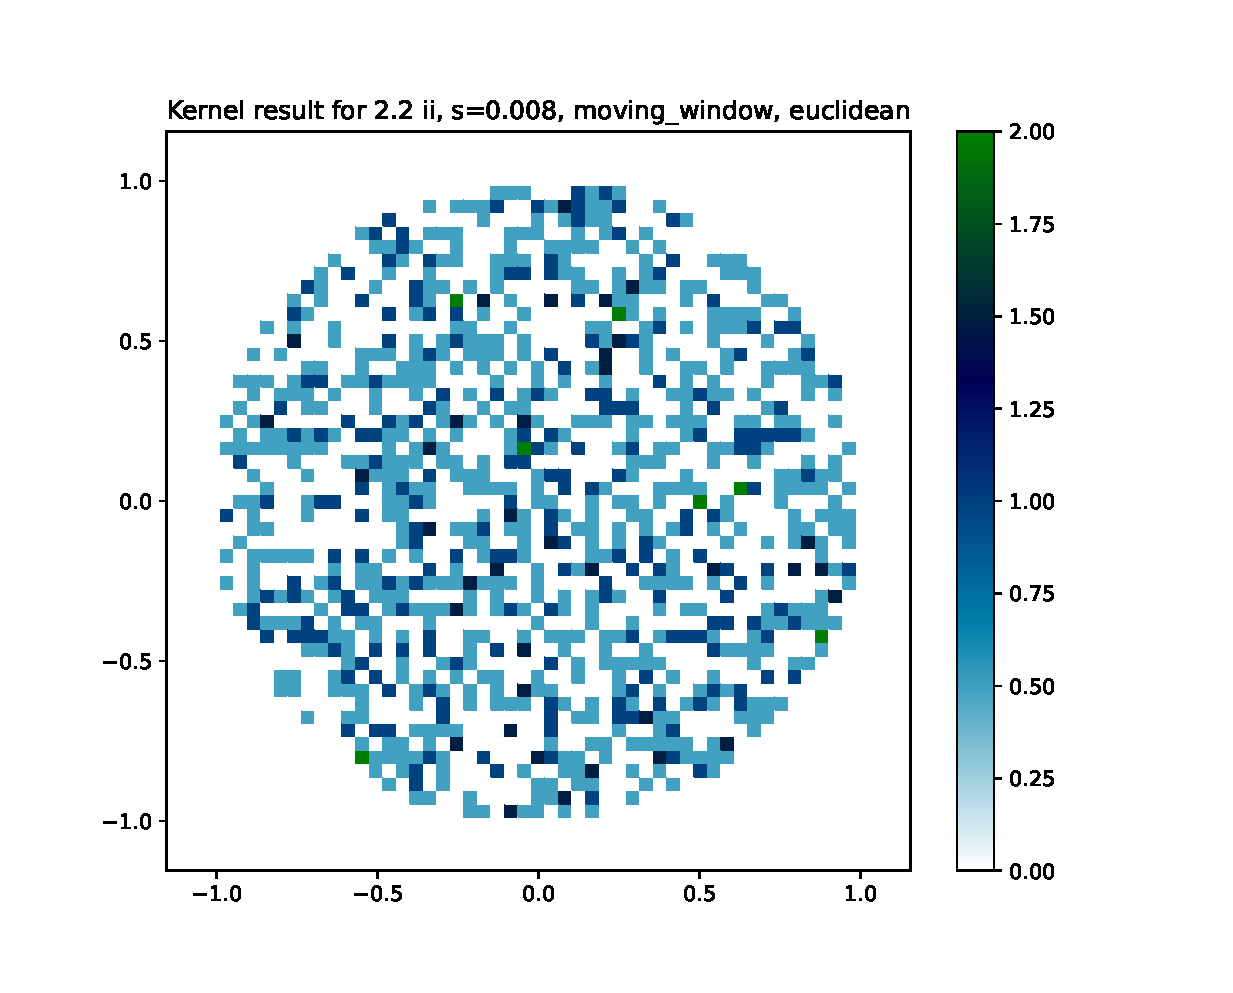
\includegraphics[height=8cm]{comparisons//Kernel_result_2-2ii_s_0-008_moving_window_euclidean.eps} \hspace*{-1.5cm}
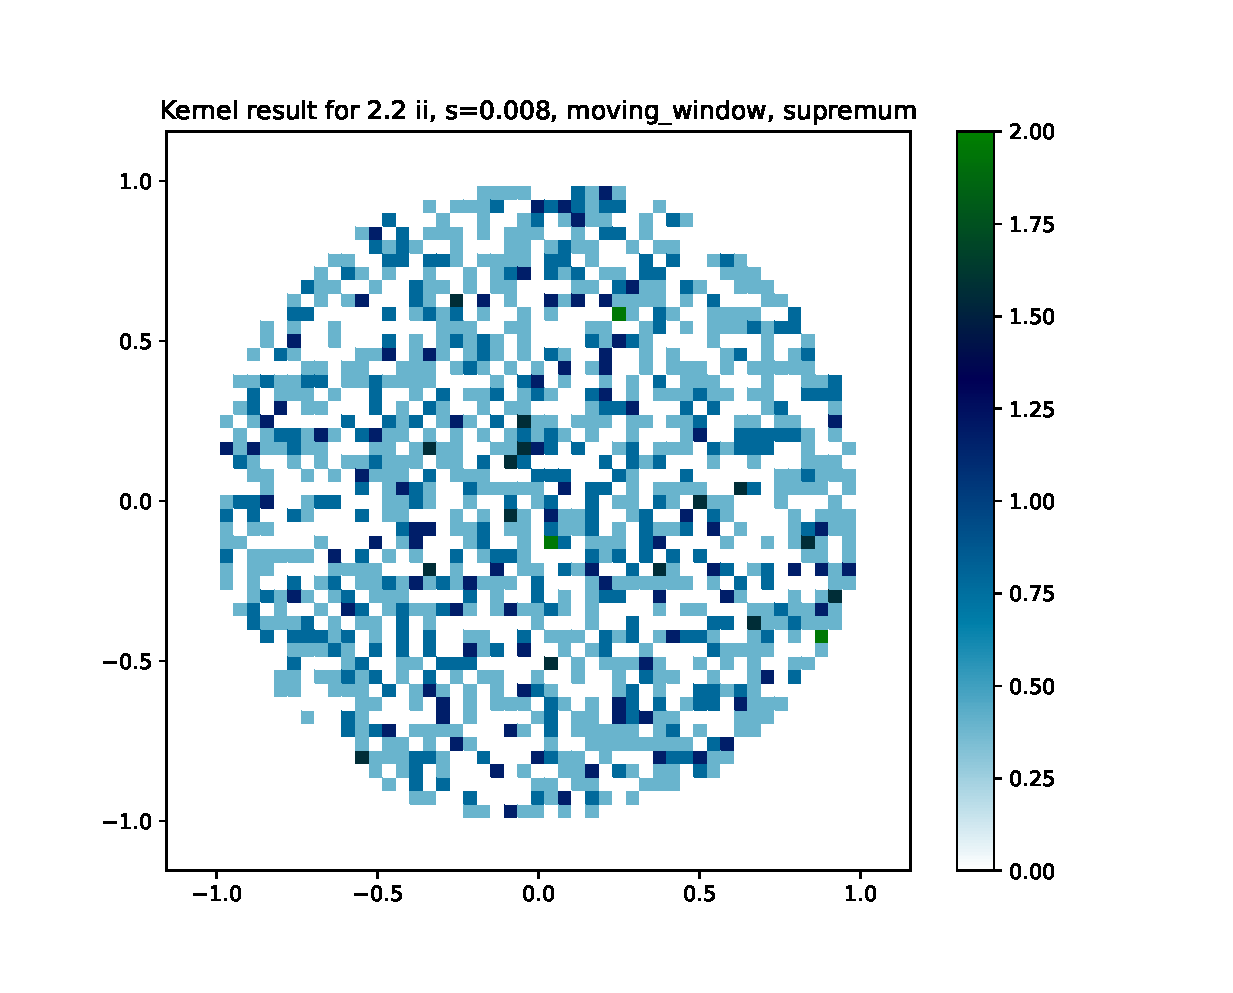
\includegraphics[height=8cm]{comparisons//Kernel_result_2-2ii_s_0-008_moving_window_supremum.eps} \vspace*{-2em} \\
What we see is that the choice of norm is seemingly less influencial, and that with decreasing $s$, the accuracy of the estimation seems to firstly grow but then decrease. \\
\noindent Secondly, we compare the results of Moving Window kernel with Gaussian kernel under Euclidean norm for different $s$: \\
\hspace*{-1.5cm}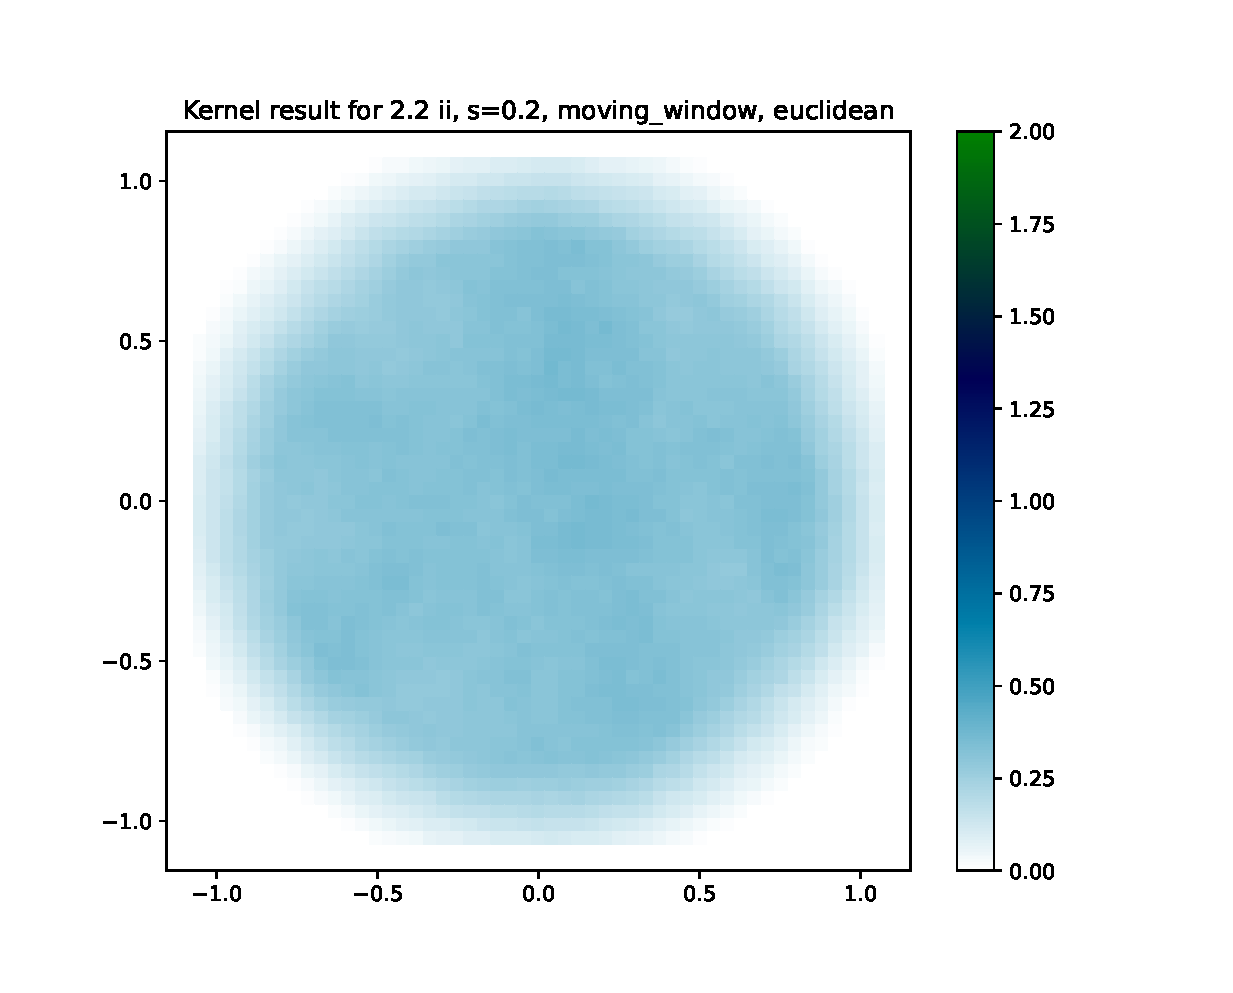
\includegraphics[height=8cm]{comparisons//Kernel_result_2-2ii_s_0-2_moving_window_euclidean.eps} \hspace*{-1.5cm}
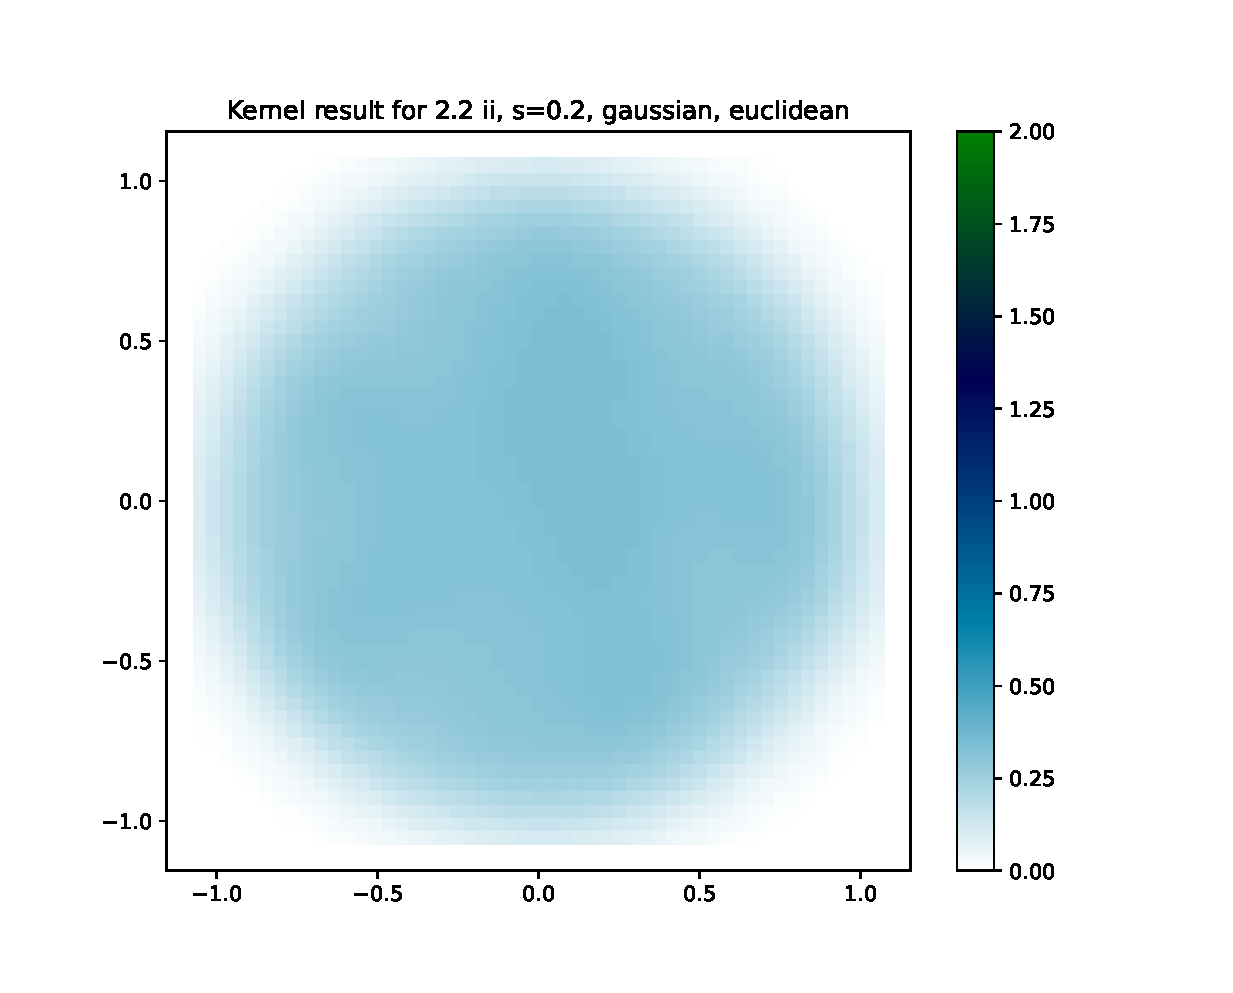
\includegraphics[height=8cm]{comparisons//Kernel_result_2-2ii_s_0-2_gaussian_euclidean.eps} \vspace*{-3em} \\
\hspace*{-1.5cm}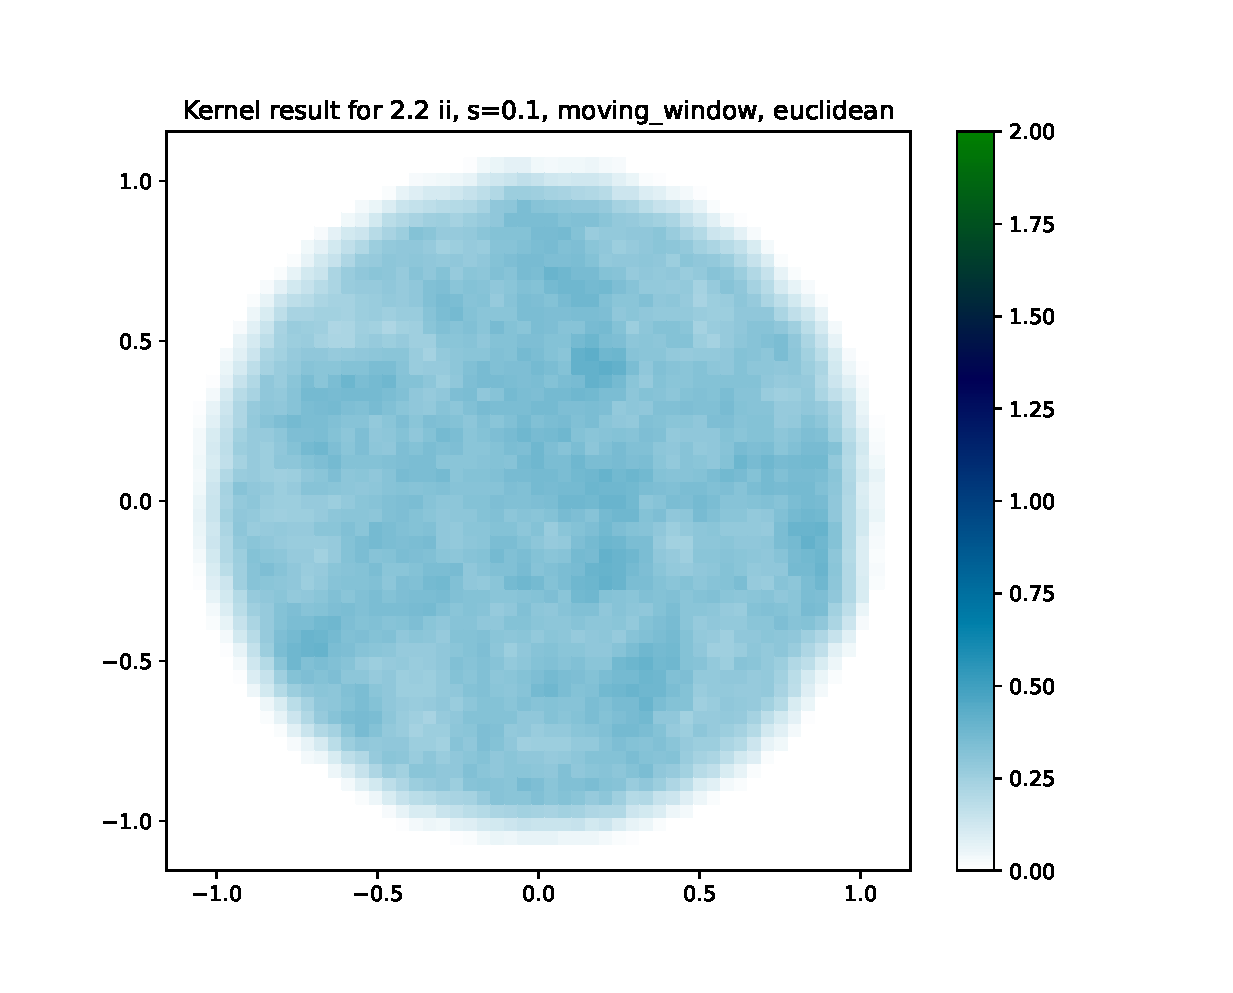
\includegraphics[height=8cm]{comparisons//Kernel_result_2-2ii_s_0-1_moving_window_euclidean.eps} \hspace*{-1.5cm}
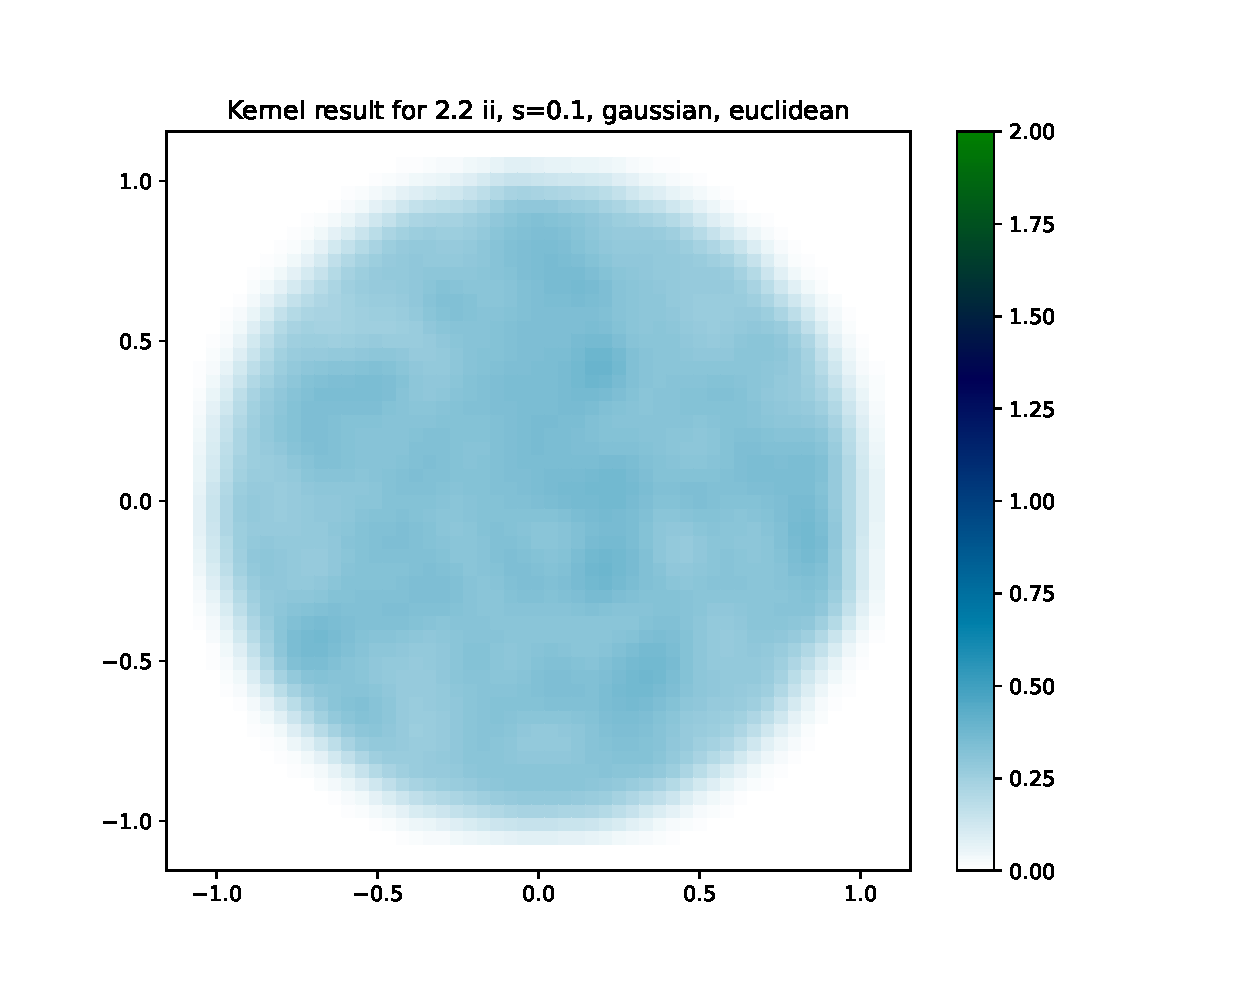
\includegraphics[height=8cm]{comparisons//Kernel_result_2-2ii_s_0-1_gaussian_euclidean.eps} \vspace*{-3em}  \\
\hspace*{-1.5cm}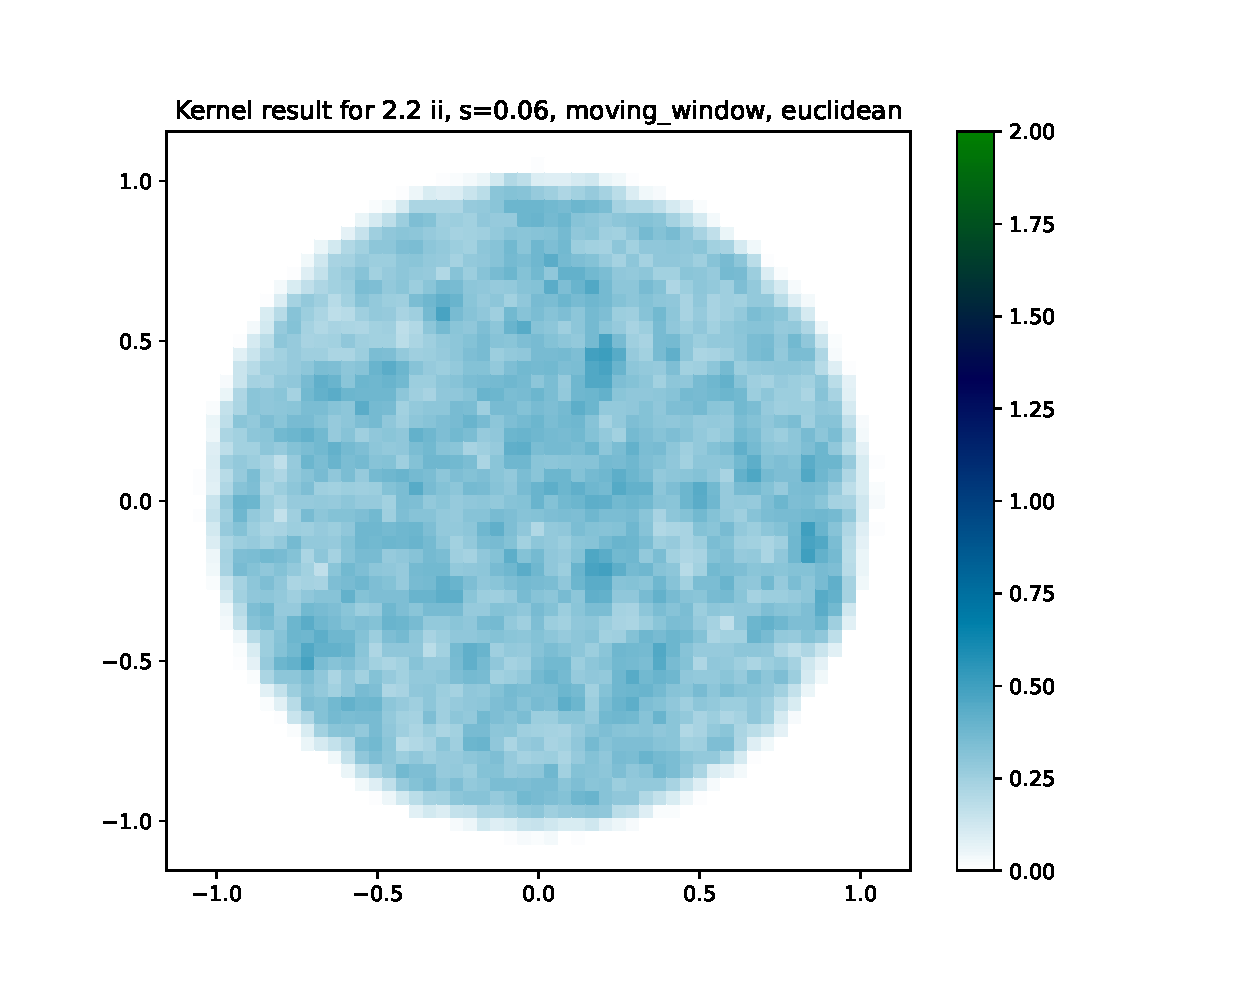
\includegraphics[height=8cm]{comparisons//Kernel_result_2-2ii_s_0-06_moving_window_euclidean.eps} \hspace*{-1.5cm}
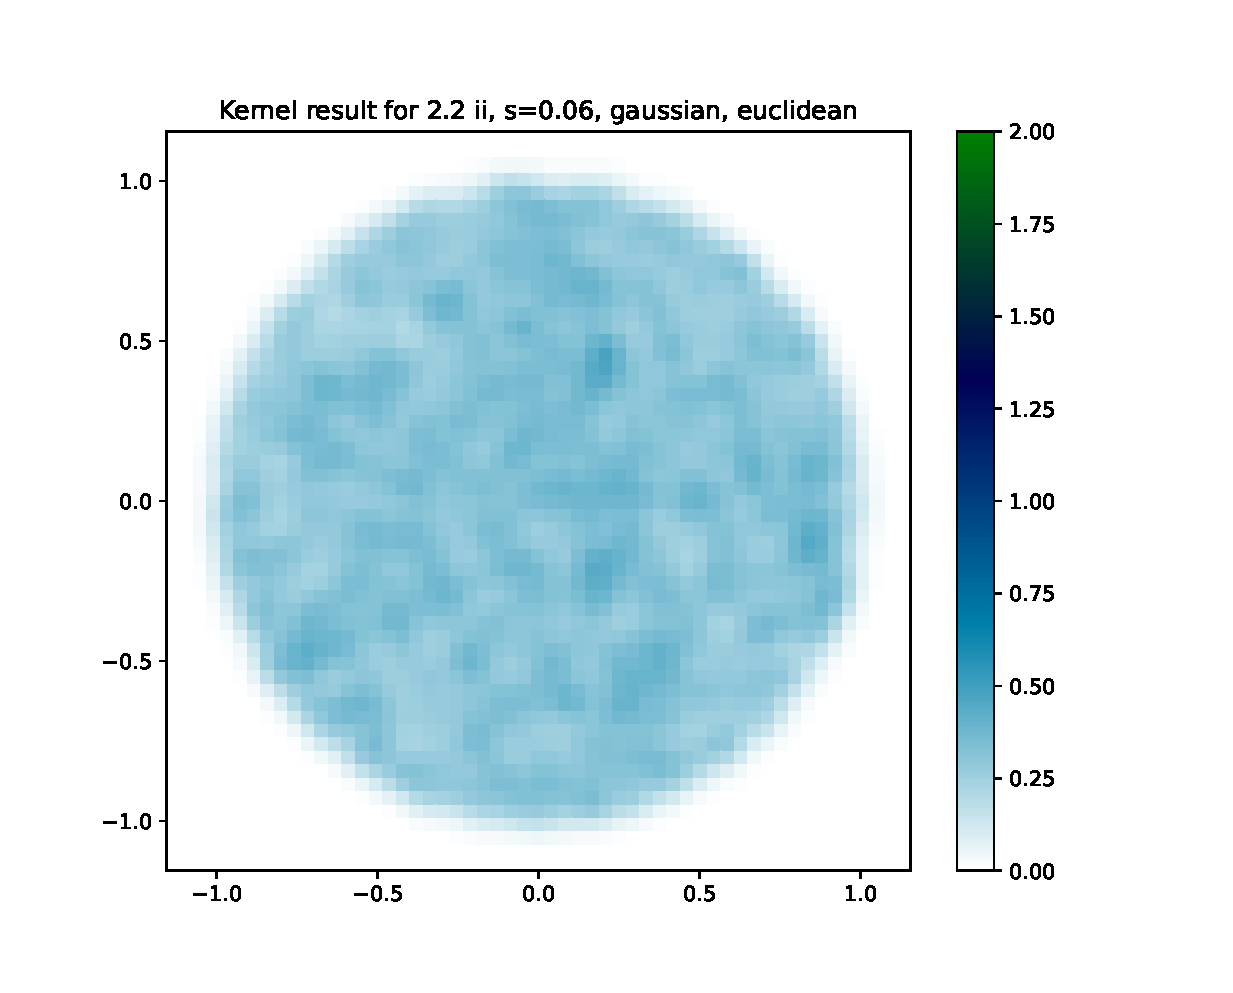
\includegraphics[height=8cm]{comparisons//Kernel_result_2-2ii_s_0-06_gaussian_euclidean.eps}  \\
\hspace*{-1.5cm}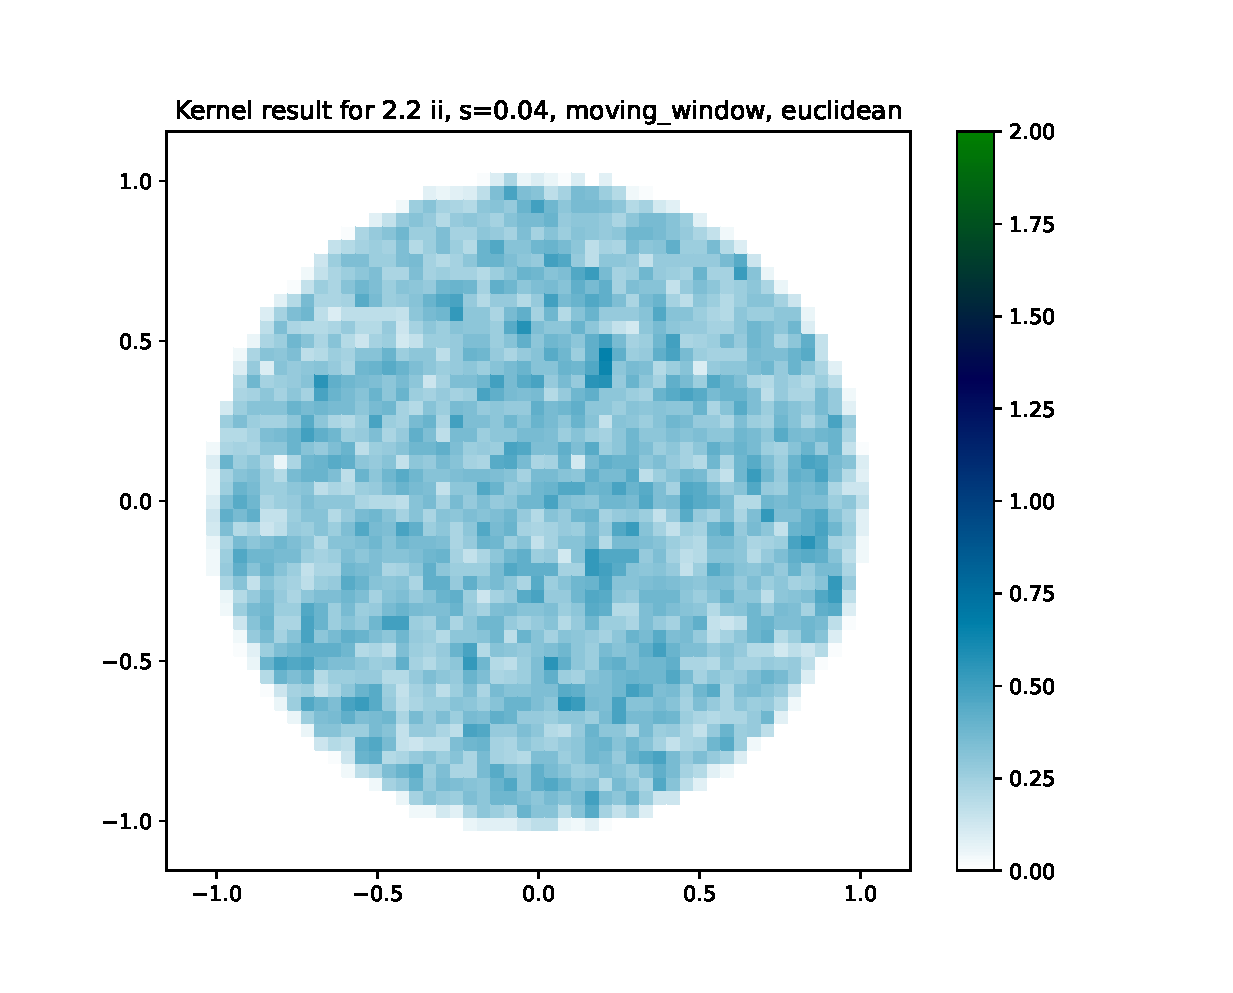
\includegraphics[height=8cm]{comparisons//Kernel_result_2-2ii_s_0-04_moving_window_euclidean.eps} \hspace*{-1.5cm}
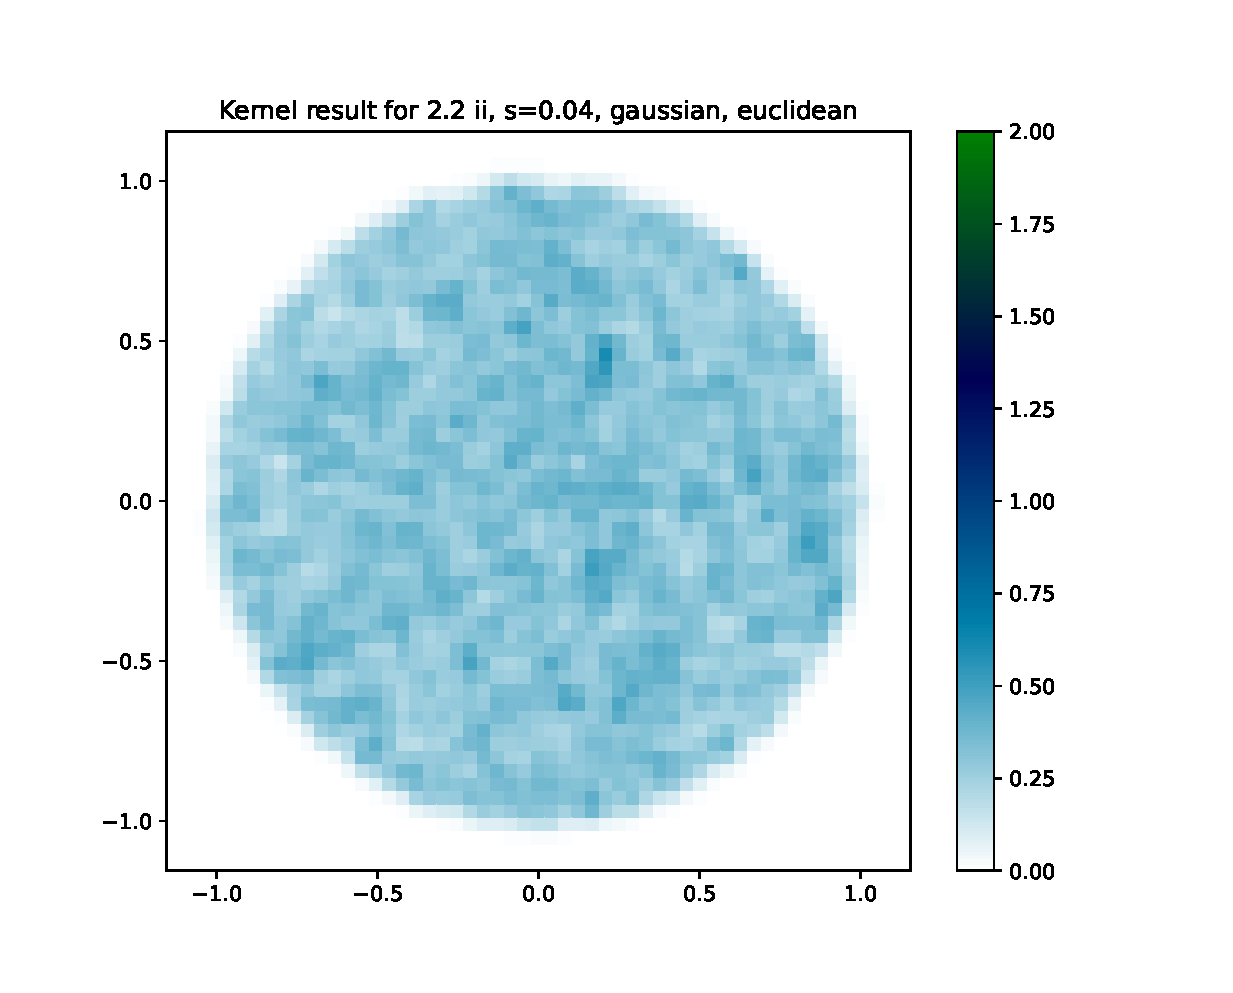
\includegraphics[height=8cm]{comparisons//Kernel_result_2-2ii_s_0-04_gaussian_euclidean.eps}  \\
\hspace*{-1.5cm}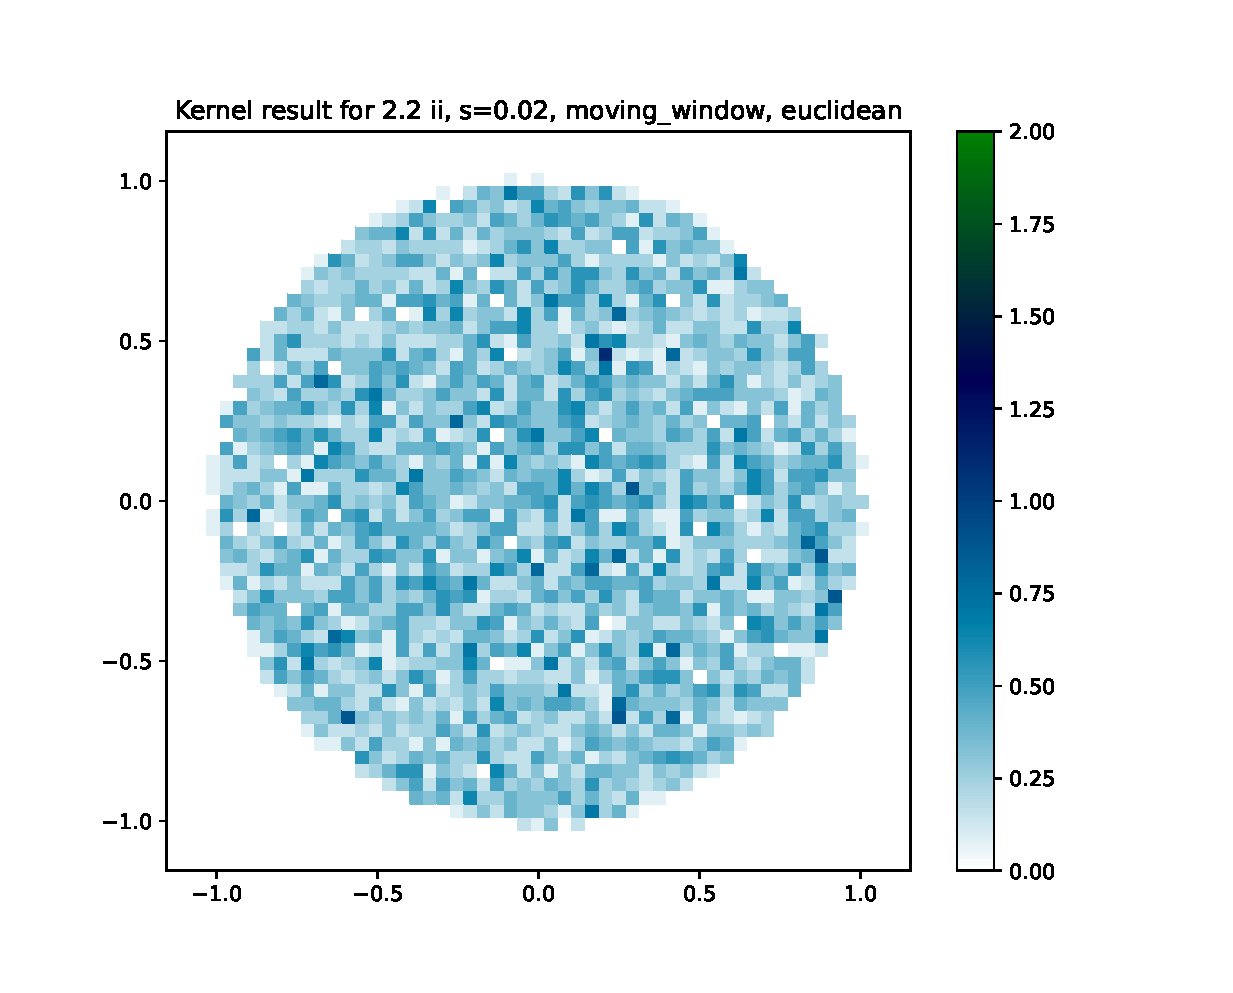
\includegraphics[height=8cm]{comparisons//Kernel_result_2-2ii_s_0-02_moving_window_euclidean.eps} \hspace*{-1.5cm}
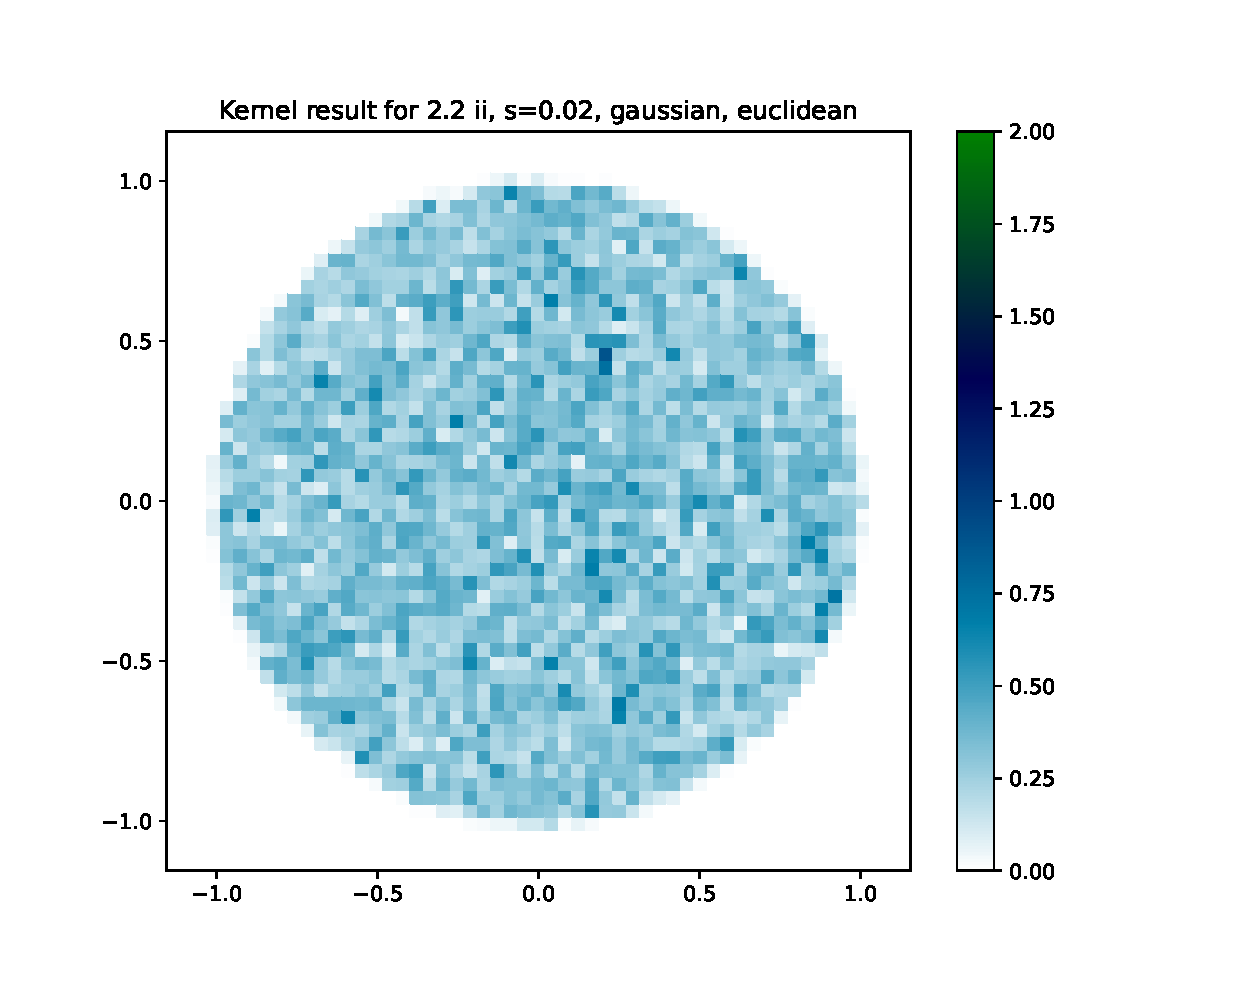
\includegraphics[height=8cm]{comparisons//Kernel_result_2-2ii_s_0-02_gaussian_euclidean.eps}  \\
\hspace*{-1.5cm}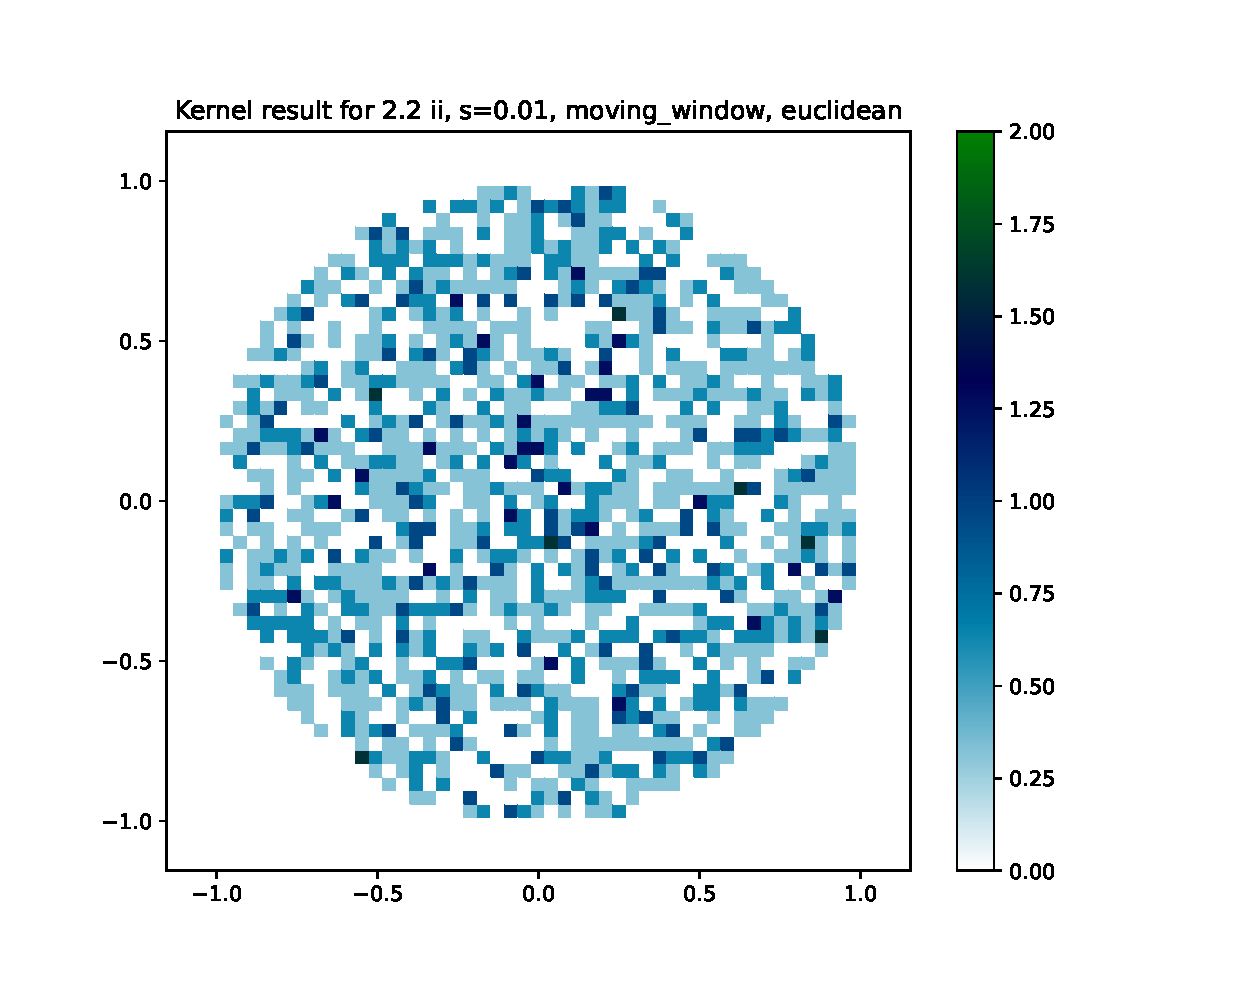
\includegraphics[height=8cm]{comparisons//Kernel_result_2-2ii_s_0-01_moving_window_euclidean.eps} \hspace*{-1.5cm}
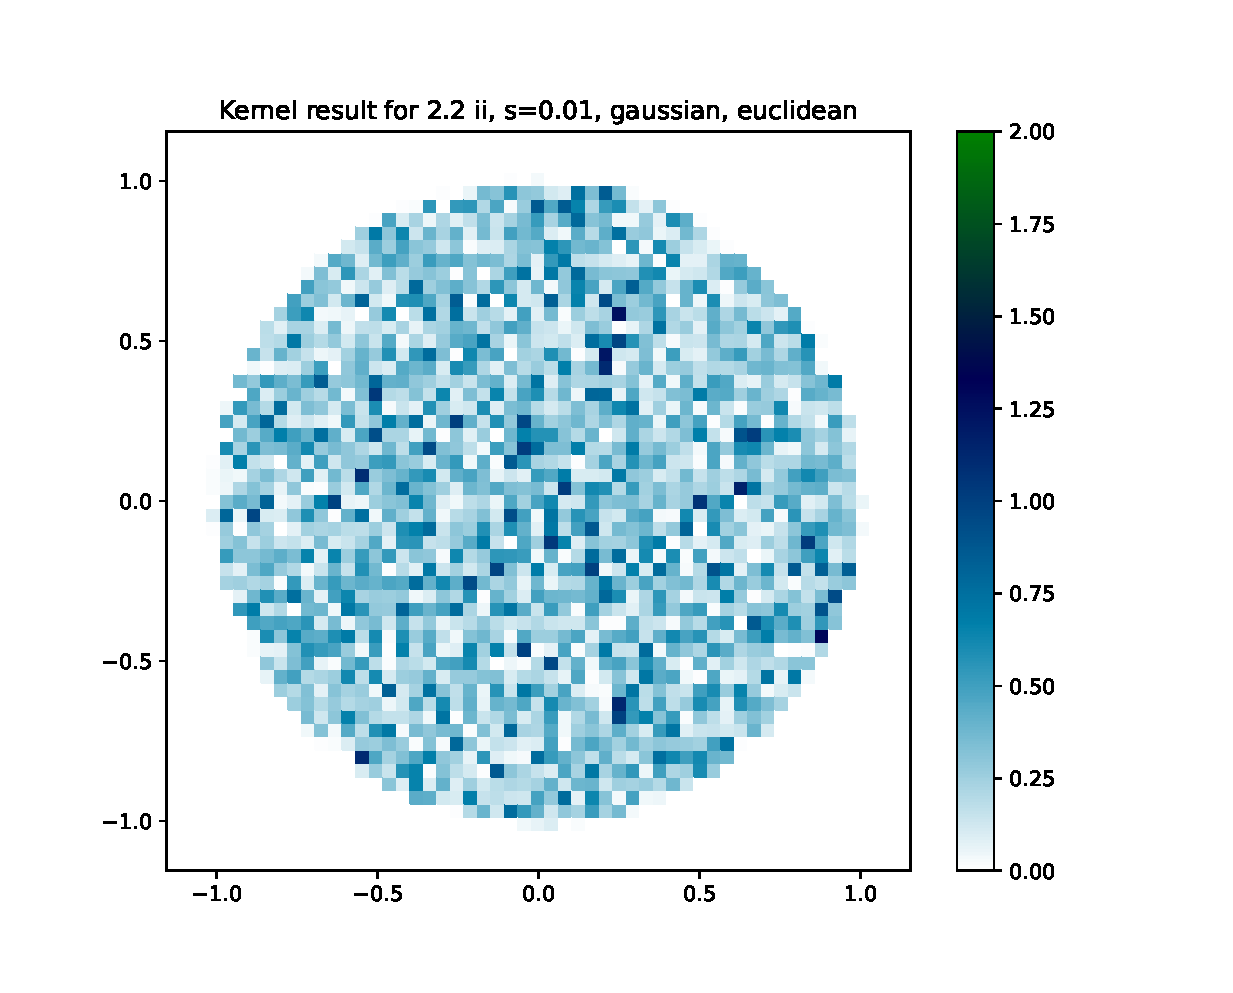
\includegraphics[height=8cm]{comparisons//Kernel_result_2-2ii_s_0-01_gaussian_euclidean.eps}  \\
\hspace*{-1.5cm}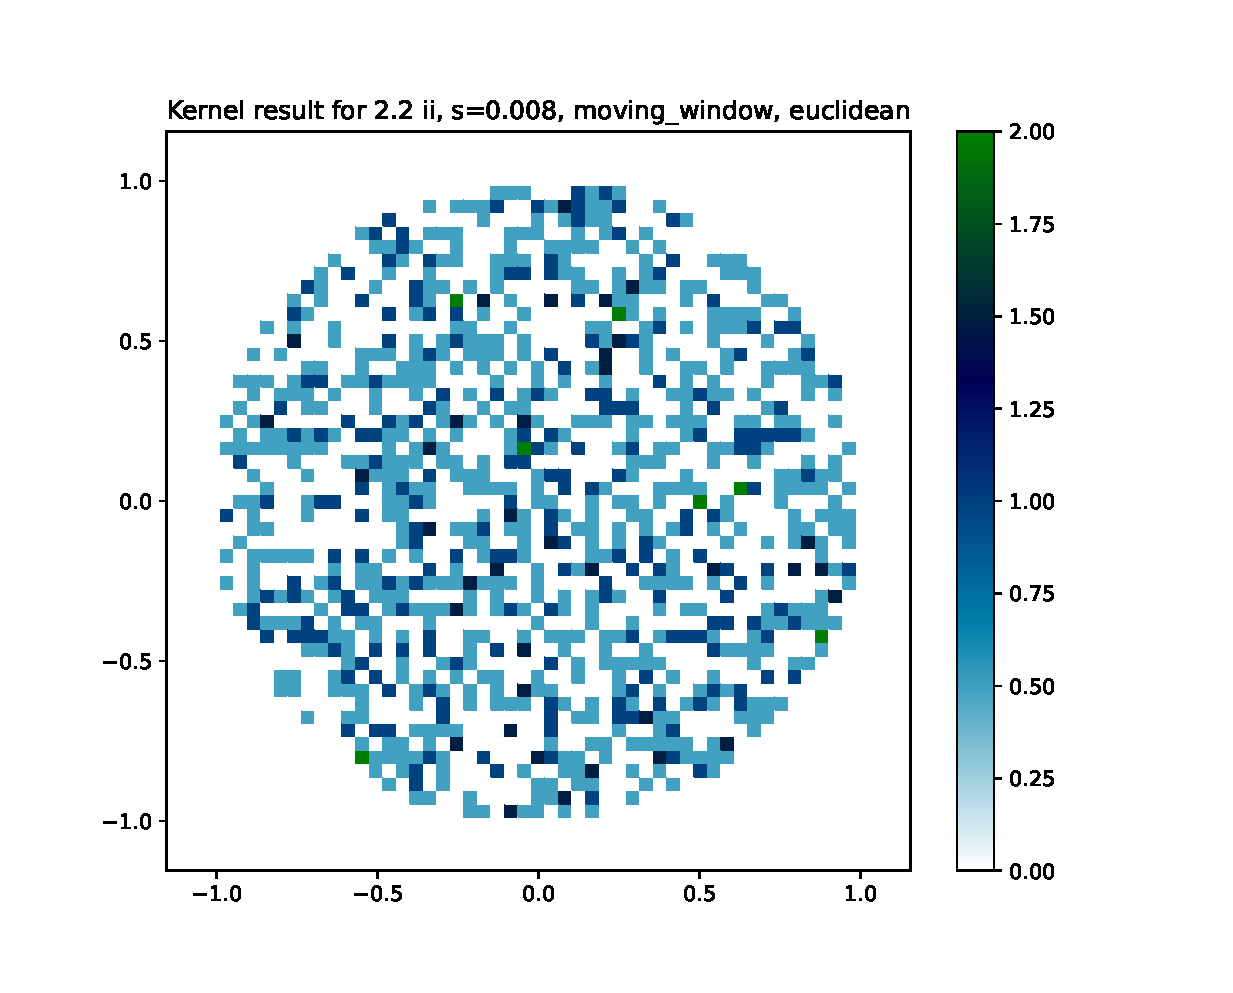
\includegraphics[height=8cm]{comparisons//Kernel_result_2-2ii_s_0-008_moving_window_euclidean.eps} \hspace*{-1.5cm}
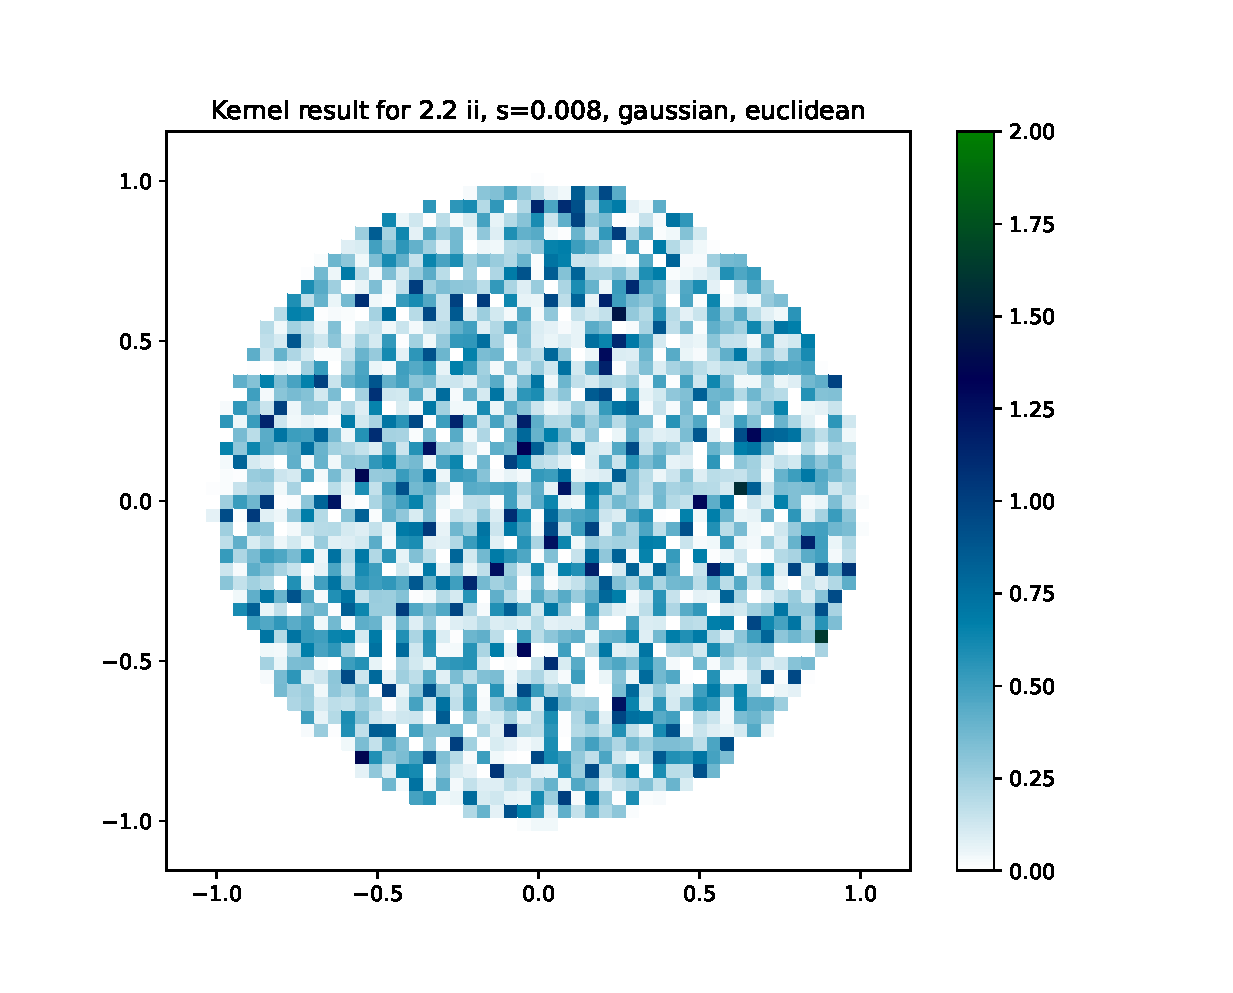
\includegraphics[height=8cm]{comparisons//Kernel_result_2-2ii_s_0-008_gaussian_euclidean.eps}  \\
Roughly speaking, the Gaussian kernel seems to outperform the Moving Window Kernel, since the plots of Gaussian kernel are "blurer". \vspace*{0.8em}\\
Let us denote $h$ as the density of the unit Euclidean ball in $\mathbb{R}^2$. \\
To take a closer look at the comparison between Moving Window and Gaussian kernels as well as between $||\cdot ||_2$ and $||\cdot ||_{\infty}$, we also implement a function that very roughly calculates $||h-h_{K,D,s}||_{L_1}$ by treating the $h_{K,D,s}$ values of all points in a grid as the same. The resuls are as follows: \vspace*{-0.6cm}\\

\begin{multicols}{2}
\begin{center}
Rough $L_1$-Norm Comparison  between Moving Window $\&$ Gaussian under $||\cdot||_2$ \vspace*{1em} \\
\begin{tabular}{ccc}

\hline  

$s$  &Moving Window              &Gaussian   \\
\hline  

0.008	    &2.54605   &2.0962 \\
0.01	    &1.68825   &2.53684 \\
0.02	    &4.53346   &6.16157 \\
0.03	    &7.55802   &9.56693 \\
0.04	    &9.37843   &12.88424 \\
0.06	    &14.4997   &19.32132 \\
0.08	    &19.76346   &25.22606 \\
0.1	    &24.28602   &30.50908 \\
0.2	    &42.96891   &52.6677 \\

\hline 
\end{tabular}

\end{center}

\begin{center}

Rough $L_1$-Norm Comparison  between $||\cdot ||_2$ and  $||\cdot ||_{\infty}$ for Moving Window kernel \vspace*{1em} \\
\begin{tabular}{ccc}

\hline  

$s$  &$||\cdot||_2$              &$||\cdot||_{\infty}$   \\
\hline  

0.008	    &2.54605   &2.07668 \\
0.01	    &1.68825   &2.2102 \\
0.02	    &4.53346   &5.29291 \\
0.03	    &7.55802   &8.46946 \\
0.04	    &9.37843   &11.04753 \\
0.06	    &14.4997   &16.35089 \\
0.08	    &19.76346   &22.89573 \\
0.1	    &24.28602   &27.41789 \\
0.2	    &42.96891   &47.2122 \\

\hline 
\end{tabular}
\end{center}

\end{multicols}

From the above tables we can see that...

\end{document}